\documentclass[a4paper]{article}
\usepackage[
    lecture,
    course={Lineare Algebra~I},
    code={V1G3},
    lecturer={Prof.~Dr.\ Jan Schröer},
    term={WS~2021/2022}
]{tienuni}

\usetikzlibrary{cd}

\overfullrule3cm

\begin{document}
\maketitle
\tableofcontents

\section{Grundlagen}

\subsection{Mengen}

Wir wollen uns mit einer sehr naiven, aber für unsere Zwecke ausreichenden, Mengenbegriff beschäftigen. Was eine Menge wirklich ist, erfahren wir von den Logikern und Mengentheoretikern.

\begin{definition}[naive Menge]
    Eine Menge~$M$ ist eine Zusammenfassung von verschiedenen Objekten, welche dann Elemente genannt werden, zu einem Objekt.
\end{definition}

\begin{example}\leavevmode
    \begin{itemize}
        \item $\N \coloneqq \mset{0, 1, 2, \dots}$, die Menge der \emph{natürliche Zahlen}. In dieser Vorlesung gehört die Null dazu.
        \item $\Z \coloneqq \mset{\dots, -2, -1, 0, 1, 2, \dots}$, die Menge der \emph{ganze Zahlen}.
        \item $\Q \coloneqq \mset{a/b \mid a, b \in \Z, b \geq 1}$, die Menge der \emph{rationale Zahlen}.
        \item $\R$,~die Menge der \emph{rationalen Zahlen}.
        \item $\C$,~die Menge der \emph{komplexen Zahlen}.
        \item $\varnothing$,~die leere Menge, die per Definition keine Elemente enthält.
    \end{itemize}
\end{example}

\begin{notation}[Quantoren, Mengenschreibweise, Relationen]
    Einige häufig verwendete Symbole
    \begin{itemize}
        \item $(\dots) \coloneqq (\dots)$ definiert das, was links steht, durch das, was rechts steht.
        \item $\forall$~bedeutet "`für alle"'.
        \item $\exists$~bedeutet "`es existiert"'.
        \item Wenn~$M$ eine Menge ist, bezeichnet $\abs{M}$ die Anzahl der Elemente in~$M$ (\emph{Kardinalität}). Für die leere Menge ist $\abs{\varnothing} = 0$.
        \item Eine Menge~$M$ heißt \emph{$n$"~elementig}, falls~$\abs{M} = n$ ($n \geq 0$).
        \item Allgemein notieren wir Mengen bspw.\ durch
              \begin{equation*}
                  \mset{21, 35} = \mset{x \in \N \mid 5 \leq x \leq 40, 7 \mid x, x \in \mset{7, 14, 28}}.
              \end{equation*}

              \begin{itemize}
                  \item[$\mset{\;}$] sind Mengenklammern.
                      \item[$\mid$]steht oft für "`mit der Eigenschaft"'. In unserem Beispiel heißt das "`alle $x \in \N$ mit der Eigenschaft, dass \dots"'
                  \item[$,$] steht oft für "`und"', eine logische Verknüpfung der Bedingungen bzw.\ Eigenschaften.
                  \item[$\in$] steht für "`ist Element von"'. Hingegen ist~$\notin$~"`ist kein Element von"'.
                  \item[$=$] steht für "`gleich"', d.\,h.\ links und rechts steht das gleiche und können gegenseitig ausgetauscht werden. Analog ist $\neq$~"`ungleich"'.
              \end{itemize}
        \item $\leq$,~$<$, $\geq$,~$>$ sind "`kleiner gleich"', "`(echt) kleiner"', "`größer gleich"', "`(echt) größer"'.
    \end{itemize}
\end{notation}

\begin{remark}
    Die Reihenfolge und Vielfachheit der Elemente in der Aufzählung von Mengen ist egal. Deshalb ist $\mset{1, 2, 3} = \mset{2, 1, 3} = \mset{1, 1, 3, 2, 3}$.
\end{remark}

\begin{definition}[Teilmenge]
    Seien $A$~und~$B$ Mengen. Dann ist
    \begin{itemize}
        \item $A$~eine \emph{Teilmenge} von~$B$, falls $x \in B$ für alle~$x \in A$, geschrieben $A \subseteq B$, und
        \item $A$~eine \emph{echte Teilmenge} von~$B$, falls $A \subseteq B$, aber~$A \neq B$, geschrieben $A \subset B$.
    \end{itemize}
\end{definition}

\begin{remark}
    Für jede Menge~$M$ gilt $\varnothing \subseteq M$, aber $\varnothing \in M$ im Allgemeinen nicht.
\end{remark}

Weiterhin definieren wir

\begin{definition}[Mengenoperatoren]
    Für Mengen $A$~und~$B$ seien
    \begin{itemize}
        \item $A \cap B \coloneqq \mset{x \mid x \in A, x \in B}$ der \emph{Durchschnitt} von $A$~und~$B$,
        \item $A \cup B \coloneqq \mset{x \mid x \in A \text{ oder } x \in B}$ die \emph{Vereinigung} von $A$~und~$B$,
        \item $A \setminus B \coloneqq \mset{x \mid x \in A, x \notin B}$ die \emph{Mengendifferenz} von $A$~und~$B$,
        \item $\powerset(A) \coloneqq \mset{U \mid U \subseteq A}$ die \emph{Potenzmenge} von~$A$.
    \end{itemize}
\end{definition}

\begin{definition}[Indexmenge]
    Sei $I$~eine \emph{Indexmenge}, d.\,h.\ für jedes~$i \in I$ ist $A_i$~eine Menge. Dann sind
    \begin{equation*}
        \bigcap_{i \in I} A_i \coloneqq \mset{x \mid x \in A_i \text{ für alle } i \in I} \qquad\text{und}\qquad \bigcup_{i \in I} A_i \coloneqq \mset{x \mid \text{es gibt ein } i \in I \text{ mit } x \in A_i}
    \end{equation*}
    der \emph{Durchschnitt} bzw.\ \emph{Vereinigung} der Mengen~$A_i$ über die Indexmenge~$I$.
\end{definition}

\begin{example}\leavevmode
    \begin{itemize}
        \item $\powerset(\mset{1, 2}) = \mset{\varnothing, \mset{1}, \mset{2}, \mset{1, 2}}$ ist 4"~elementig.
        \item $\mset{1, 2, 3} \cup \mset{2, 3} = \mset{1, 2, 3}$.
        \item $\mset{1, 2} \setminus \mset{1, 3} = \mset{2}$. Die Differenzmenge~$A \setminus B$ nimmt $B$ von~$A$ weg.
        \item $\varnothing \cup \mset{1, 2} = \mset{1, 2} \neq \mset{\varnothing, 1, 2} = \mset{\varnothing} \cup \mset{1, 2}$. Die Vereinigung mit der leeren Menge macht nichts.
        \item $\mset{\varnothing, \mset{1, 2, 3, 4}}$ ist 2"~elementig, wohingegen $\mset{\varepsilon, 1, 2, 3, 4}$ 5"~elementig ist.
    \end{itemize}
\end{example}

\begin{definition}[Paar]
    Ein \emph{Paar} (oder \emph{2"~Tupel}) besteht aus der Angabe eines ersten Elements~$a$ und eines zweiten Elements~$b$. Wir schreiben~$(a, b)$.
\end{definition}

\begin{remark}
    Bei Paaren ist (im Gegensatz zu Mengen) die Reihenfolge wichtig. Es gilt $(a, b) = (b, a)$ genau dann, wenn~$a = b$: \emph{Achtung}: $(a, a) \neq \mset{a, a} = \mset{a}$.
\end{remark}

\begin{definition}[\textsc{kartesisches} Produkt, Tupel]
    Das \emph{\textsc{kartesische} Produkt} zweier Mengen $A$~und~$B$ ist $A \times B \coloneqq \mset{(a, b) \mid a \in A, b \in B}$.

    Für Mengen $A_1, A_2, \dots, A_n$ ist das \emph{\textsc{kartesische} Produkt}
    \begin{equation*}
        A_1 \times \dots \times A_n \coloneqq \mset{(a_1, \dots, a_n) \mid a_i \in A_i \text{ für } 1 \leq i \leq n},
    \end{equation*}
    dessen Elemente \emph{$n$"~Tupel} genannt werden.

    Sei~$A$ eine Menge und~$n \geq 1$. Dann ist
    \begin{equation*}
        A^n \coloneqq \underbrace{A \times \dots \times A}_{n \text{ mal}}
    \end{equation*}
    das \emph{$n$"~fache \textsc{kartesische} Produkt} von~$A$.
\end{definition}

\begin{remark}
    Zwei Tupel sind gleich, wenn sie gleich viele \emph{Einträge} bzw.\ \emph{Komponenten} haben und wenn an jeder Stelle die Komponenten gleich sind.
\end{remark}

\begin{notation}
    Die $n$"~Tupel $(a_1,a_2,\dots,a_n)$ schreiben wir oft auch senkrecht auf:
    \begin{equation*}
        \p{a_1\\a_2\\\vdots\\a_n}
    \end{equation*}
\end{notation}

\begin{example}
    Sind $A$,~$B$ und~$C$ Mengen, dann sind die Elemente in~$A \times B \times C$ 3"~Tupel der Form $(a, b, c)$, während die Elemente in~$(A \times B) \times C$ 2"~Tupel der Form $((a, b), c)$.
\end{example}

\subsection{Logik}

\begin{definition}[Implikation, Äquivalenz]
    Seien $A$,~$B$ und~$C$ Aussagen. Dann bedeuten
    \begin{itemize}
        \item $A \implies B$ "`$A$~impliziert~$B$"', "`aus~$A$ folgt~$B$"',
        \item $A \iff B$ "`$A$~genau dann, wenn~$B$"', "`$A$~und~$B$ sind äquivalent"', d.\,h.\ $A \implies B$ und $B \implies A$,
        \item $\neg A$, "`nicht~$A$"'.
    \end{itemize}
\end{definition}

Zwei Schlussregeln, die wir oft verwenden werden:

\begin{theorem}[Syllogismus, Kontraposition]\label{thm:deductionrules}\leavevmode
    \begin{itemize}
        \item Aus~$A \implies B$ und~$B \implies C$ folgt~$A \implies C$ (\emph{Syllogismus}).
        \item Es gilt~$A \implies B$ genau dann, wenn~$\neg B \implies \neg A$ (\emph{Kontraposition}).
    \end{itemize}
\end{theorem}

\begin{example}
    \begin{gather*}
        \underbrace{\text{"`Wenn es regnet,}}_{\displaystyle A}\; \underbrace{\text{ist die Straße nass."'}}_{\displaystyle B} \qquad (A \implies B) \\
        \shortintertext{ist äquivalent zu} \\
        \underbrace{\text{"`Wenn die Straße nicht nass ist,}}_{\displaystyle\neg B}\; \underbrace{\text{dann regnet es nicht."'}}_{\displaystyle\neg A} \qquad (\neg B \implies \neg A)
    \end{gather*}
\end{example}

\subsubsection{Beweis durch Induktion}

Für jedes natürliche~$n \geq 1$ sei $A(n)$~eine Aussage. Wenn das Ziel ist, $A(n)$ für alle~$n \geq 1$ zu zeigen, dann kann \emph{vollständige Induktion} helfen. Die Beweisstrategie:
\begin{itemize}
    \item \emph{Induktionsanfang}: Wir zeigen, dass $A(1)$~richtig ist.
    \item \emph{Induktionsschritt}: Wir nehmen an, dass $A(n)$~richtig ist. Damit beweisen wir, dass auch $A(n+1)$~richtig ist.
\end{itemize}

Das Beweisprinzip basiert auf dem Dominoeffekt: Mit dem Induktionsanfang ist~$A(1)$ wahr. Mit dem Induktionsschritt folgt aus~$A(1)$ auch~$A(2)$. Wieder mit dem Induktionsschritt folgt aus~$A(2)$ auch~$A(3)$ usw. Damit haben wir die Aussagen~$A(n)$ für alle~$n \geq 1$ gezeigt.

\begin{example}\leavevmode
    \begin{itemize}
        \item Für alle~$n \geq 1$ gilt $A(n)\colon \sum_{k=1}^n (2k-1) = n^2$.
              \begin{itemize}
                  \item \emph{Induktionsanfang} ($n = 1$): $2 \cdot 1 - 1 = 1^2$ ist wahr und deshalb auch~$A(1)$.
                  \item \emph{Induktionsschritt}: Es gilt
                        \begin{equation*}
                            \sum_{k=1}^{n+1} (2k-1) = \paren*{\sum_{k=1}^n (2k-1)} + (2(n+1) - 1) = n^2 + 2n + 1 = (n+1)^2.
                        \end{equation*}
                        Dabei verwendeten wir für die zweite Gleichheit die Induktionsvoraussetzung. Folglich gilt~$A(n+1)$.
              \end{itemize}
        \item Ein falscher Induktionsbeweis: Wir behaupten, dass $A(n)\colon (7 \text{ teilt } 10^n)$ für alle~$n \geq 1$ gilt.
              \begin{itemize}
                  \item \emph{Induktionsschritt}: Angenommen $A(n)$ ist wahr, d.\,h.\ es gilt $10^n = 7a$ für ein~$a \geq 1$ in~$\N$. Dann gilt auch $10^{n+1} = 10 \cdot 10^n = 10 \cdot 7a$. Also gilt~$A(n+1)$.
                  \item \emph{Induktionsanfang}: Aber~$A(1)$ ist falsch!
              \end{itemize}
    \end{itemize}
\end{example}

\subsubsection{Beweis durch Widerspruch}

Das Beweisprinzip ist, das Gegenteil der Behauptung anzunehmen und das auf einen Widerspruch mit der Voraussetzung zu führen. Folglich war die Annahme falsch und die Behauptung richtig.

\begin{example}
    \emph{Behauptung}: $\sqrt{2} \notin \Q$.

    \emph{Beweis}: Angenommen $\sqrt{2} \in \Q$, d.\,h.\ Es gibt $a, b \in \Z$, $b \geq 1$ mit~$\sqrt{2} = a/b$. Wir können annehmen, dass $a$~und~$b$ teilerfremd sind (also der Bruch vollständig gekürzt ist).

    Quadrieren liefert $2 = a^2/b^2 \iff 2b^2 = a^2$. Damit sind $a^2$~und~$a$ durch $2$~teilbar, insbesondere auch~$a^2$ durch $2\cdot2 = 4$ teilbar. Somit teilt~$4$ auch~$2b^2$, also sind $b^2$~und~$b$ auch durch $2$~teilbar (aufgrund der Eindeutigkeit der Primfaktorzerlegung). Das bedeutet, dass $a$~und~$b$ durch $2$~teilbar sind, was im Widerspruch zur Teilerfremdheit steht.
\end{example}

\subsubsection{Gleichheit von Mengen}

\begin{remark}
    Zwei Mengen sind \emph{gleich}, wenn sie dieselben Elemente besitzen.
\end{remark}

Seien $A$~und~$B$ zwei Mengen. Um zu beweisen, dass~$A=B$ ist, muss man zum Einen~$A \subseteq B$ und zum Anderen~$B \subseteq A$ zeigen. Der Beweis ist im Regelfall also zweiteilig!

\subsection{Abbildungen}

Die Idee hinter Abbildungen ist es, Mengen in Beziehung zu setzen.\footnote{Eigentlich sind es die \emph{Relationen} die das erfüllen, wovon Abbildungen eine spezielle Form sind.}

\begin{definition}[Abbildung]
    Seien $X$~und~$Y$ Mengen. Eine \emph{Abbildung}~$f$ von~$X$ nach~$Y$ ist eine Vorschrift, durch die jedem~$x \in X$ genau ein~$f(x) \in Y$ zugeordnet wird.\footnote{Die Menge~$X$ bezeichnen wir als \emph{Definitionsmenge} und $Y$~als \emph{Zielmenge}. Die Elemente aus~$X$ heißen \emph{Urbilder} oder \emph{Argumente}, die Elemente aus~$Y$ heißen \emph{Zielelemente}. Die tatsächlich angenommen Werte nennen wir \emph{Bilder} oder schlicht \emph{Werte}, und deren Menge auch \emph{Bild} oder \emph{Bildmenge}.}
\end{definition}

\begin{remark}
    Jedes~$x$ wird genau einem~$f(x)$ zugeordnet. Trotzdem ist es möglich, dass verschiedene~$x$ demselben~$f(x)$ zugeordnet werden.
\end{remark}

\begin{remark}
    Zwei Abbildungen sind gleich, wenn sie dieselben Definitions"~ und Zielmengen haben sowie elementweise bzw.\ punktweise gleich sind (d.\,h.\ deren Vorschrift dasselbe macht).
\end{remark}

\begin{notation}
    Wir schreiben $f\colon X \to Y$, $x \mapsto f(x)$. Dabei verwenden wir~$\to$ zwischen Mengen und~$\mapsto$ zwischen Elementen.
\end{notation}

\begin{definition}[Menge aller Abbildungen]
    Seien $X$~und~$Y$ Mengen. Dann ist $\map(X, Y)$~die \emph{Menge aller Abbildungen} von~$X$ nach~$Y$.
\end{definition}

\begin{example}
    Die Abbildung $f\colon \Z \to \N$, $x \mapsto x^2$ bildet jedes~$x \in \Z$ auf~$x^2 \in \N$ ab.
\end{example}

\begin{definition}[Identität]
    Sei $X$~eine Menge. Als \emph{Identität} von~$X$ bezeichnen wir die Abbildung~$\id_X\colon X \to X$, $x \mapsto x$. Es gilt also $\id_X(x) = x$ für alle~$x \in X$.
\end{definition}

\begin{definition}[Komposition von Abbildungen]
    Seien $f\colon X \to Y$ und $g\colon Y \to Z$ Abbildungen. Dann ist
    \begin{equation*}
        g \circ f\colon X \to Z,\quad x \mapsto g(f(x))
    \end{equation*}
    die \emph{Komposition} (\emph{Hintereinanderschaltung}, \emph{Verkettung}) von~$f$ und~$g$, gelesen "`$g$~verknüpft mit~$f$"', "`$g$~komponiert mit~$f$"', "`$g$~nach~$f$"' oder "`$g$~Kringel~$f$"'.
\end{definition}

\begin{notation}
    Wir schreiben auch manchmal $gf$~für~$g \circ f$.
\end{notation}

Es gilt also
\begin{equation*}
    \begin{tikzcd}
        X \ar[r, "f"] & Y \ar[r, "g"] & Z
    \end{tikzcd},
    \quad
    \begin{tikzcd}
        x \ar[r, mapsto] & f(x) \ar[r, mapsto] & g(f(x))
    \end{tikzcd}.
\end{equation*}

\begin{definition}[injektiv, surjektiv, bijektiv]
    Sei $f\colon X \to Y$ eine Abbildung. Dann ist
    \begin{itemize}
        \item $f$~\emph{text}, falls für alle $x_1 \neq x_2$ in~$X$ gilt: $f(x_1) \neq f(x_2)$,
        \item $f$~\emph{surjektiv}, falls für jedes~$y \in Y$ ein~$x \in X$ existiert, sodass $f(x) = y$ ist, und
        \item $f$~\emph{bijektiv}, falls $f$~injektiv und surjektiv ist. Dann nennen wir $f$ eine \emph{Bijektion}.
    \end{itemize}
\end{definition}

\begin{definition}[Umkehrabbildung]
    Sei $f\colon X \to Y$ eine bijektive Abbildung. Dann ist die \emph{Umkehrabbildung} $f^{-1}\colon Y \to X$ definiert durch~$f^{-1}(f(x)) \colon x$ für alle~$x \in X$ bzw.~$f(x) \in Y$.

    Es gilt dann $f^{-1} \circ f = \id_X$ und $f \circ f^{-1} = \id_Y$.
\end{definition}

Umkehrabbildungen kann es nur für Bijektionen geben. Da auch~$f^{-1}$ eine Abbildung sein soll und Abbildungen jedem~$y \in Y$ \emph{genau ein}~$x \in X$ zuordnet, müssen wir die Injektivität von~$f$ voraussetzen. Dann sind nämlich $f^{-1}(f(x_1))$ und~$f^{-1}(f(x_2))$ für~$x_1, x_2 \in X$ mit~$x_1 \neq x_2$ auch unterschiedlich. Da~$f^{-1}$ von~$Y$ nach~$X$ abbilden soll, muss $f^{-1}(y)$ für alle~$Y$ definiert werden, weshalb wir die Surjektivität voraussetzen müssen. Dann gibt es für jedes~$y \in Y$ ein~$x \in X$ mit~$y = f(x)$, sodass $f^{-1}(y) = x$ wohldefiniert\footnote{Der Begriff \emph{wohldefiniert} meint, dass ein Begriff eindeutig und widerspruchsfrei definiert ist, also weder unmöglich noch mehrdeutig ist.} ist.

Auch die Komposition der Abbildung und dessen Umkehrung ergibt Sinn: $f^{-1} \circ f$~bildet von~$X$ nach~$Y$ und wieder nach~$X$ ab, und $f \circ f^{-1}$ bildet von~$Y$ nach~$X$ und wieder nach~$Y$ ab.

\begin{example}\leavevmode
    \begin{enumerate}
        \item $f\colon \mset{1, 2, 3} \to \mset{1, 2}$ mit $1 \mapsto 1$, $2 \mapsto 1$ und $3 \mapsto 2$ ist surjektiv, aber nicht injektiv.
        \item $f\colon \mset{1, 2} \to \mset{1, 2, 3}$ mit $1 \mapsto 3$ und $2 \mapsto 1$ ist injektiv, aber nicht surjektiv.
        \item $f\colon \Z \to \Z$, $x \mapsto x-41$ ist injektiv und surjektiv, also bijektiv.
        \item $f\colon \Z \to \Z$, $x \mapsto 2x$ ist injektiv, aber nicht surjektiv (die ungeraden Zahlen werden nicht getroffen).
        \item $f\colon \Z \to \Z$ mit $2n \mapsto n$ und $2n+1 \mapsto n$ (für~$n \in \Z$) ist surjektiv, aber nicht injektiv.
        \item Seien $X$~und~$Y$ zwei endliche Mengen mit gleich vielen Elementen. Dann ist die Abbildung $f\colon X \to Y$ genau dann injektiv, wenn $f$~surjektiv ist.
        \item Die Abbildung $f\colon \mset{\text{Menschen in Bonn}} \to \N$ definiert durch $x \mapsto \text{Alter}(x)$ ist weder surjektiv (Menschen werden nicht beliebig alt) noch injektiv (zwei Menschen können dasselbe Alter haben).
        \item Für ein fixiertes $(a, b, c, d) \in \Q^4$ definieren wir $f\colon \Q^2 \to \Q^2$, $(x, y) \mapsto (ax+by, cx+dy)$. Die Abbildung $f$~ist genau dann bijektiv, wenn $ad-bc \neq 0$ gilt. Außerdem ist $f$ genau dann injektiv, wenn $f$~surjektiv ist. (Der Beweis dafür erfolgt später.)\footnote{Das ist das Matrix-Vektor-Produkt, wobei $a,b,c,d$ die Einträge einer Matrix~$A \in \Q^{2, 2}$ ist und $x,y$ die Einträge eines Vektors~$v$. Dann ist $A$~genau dann ein Isomorphismus, wenn $A$~invertierbar ist, also $ad-bc \neq 0$. Genauso ist eine quadratische Matrix genau dann ein Monomorphismus, wenn sie ein Epimorphismus ist.}
    \end{enumerate}
\end{example}

\lecturesep{12.~Oktober 2021}

\begin{definition}
    Seien $M$~und~$I$ Mengen. Dann sei
    \begin{equation*}
        M^I \coloneqq \map(I, M)
    \end{equation*}
    die \emph{Menge aller Abbildungen~$I \to M$}.
\end{definition}

\emph{Achtung}: Es sind die Abbildungen von~$I$ nach~$M$, nicht von~$M$ nach~$I$!

\begin{example}\label{ex:map:setisoproduct}
    Für $I = \mset{1, \dots, n}$ ist die Abbildung $M^I \to M^n$, $f \mapsto (f(1), \dots, f(n))$ bijektiv, wobei $M^n$~bekanntlich das $n$"~fache kartesische Produkt bezeichnet.

    Offensichtlich haben alle~$f \in M^I$ dieselben Definitions"~ und Zielmengen. Dann sind zwei Abbildungen genau dann gleich, wenn sie für jedes Argument denselben Wert liefern, d.\,h.\ wenn die Tupel ihrer Werte gleich sind. Andersherum definiert jedes Tupel eine Abbildung, denn es gibt alle möglichen Zuordnungen $I \to M$ an.\footnote{In fortgeschrittener Sprache: Die Abbildung ist ein \emph{Mengenisomorphismus}, also ein bijektiver Homomorphismus, der die Mengenstruktur (auch wenn sehr banal) erhält.}

    \emph{Achtung}: Die hier beschriebene Abbildung bildet \emph{Abbildungen}~$f$ auf \emph{$n$"~Tupel derer Werte} ab.
\end{example}

\begin{definition}[Bild, Urbild einer Menge]
    Sei $f\colon X \to Y$ eine Abbildung. Und seien $A \subseteq X$ und~$B \subseteq Y$ Teilmengen. Wir bezeichnen
    \begin{equation*}
        f(A) \coloneqq \mset{f(x) \mid x \in A} \qquad\text{und}\qquad f^{-1}(B) \coloneqq \mset{x \mid f(x) \in B}
    \end{equation*}
    als \emph{Bild} von~$A$ unter~$f$ bzw.\ \emph{Urbild} von~$B$ unter~$f$. Dahingegen ist $f(X)$ das \emph{Bild} von~$f$. Es gilt stets $f^{-1}(Y) = X$.
\end{definition}

\emph{Warnung}: Die Schreibweise~$f^{-1}(B)$ impliziert nicht, dass eine Umkehrabbildung existiert.

\begin{remark}
    Wir beachten, dass das nicht jedes~$y \in B$ ein Urbild~$\in f^{-1}(B)$ haben muss, ähnlich wie eine Abbildung nicht surjektiv sein muss. Genauso kann es mehrere Urbilder~$x_1,x_2 \in f^{-1}(B)$ mit~$x_1 \neq x_2$ zu einem Bild~$y$ mit $f(x_1) = f(x_2) = y$ geben, ähnlich wie eine Abbildung nicht injektiv sein muss.
\end{remark}

\begin{definition}[Graph]
    Der \emph{Graph} einer Abbildung $f\colon X \to Y$ ist
    \begin{equation*}
        \Gamma(f) \coloneqq \mset{(x, f(x)) \mid x \in X} \subseteq X \times Y.
    \end{equation*}
\end{definition}

Der Graph ist also eine "`Zeichnung"' der Funktion, also die Menge aller Punkte der "`Ebene"', die zur Funktion "`gehören"'.

\begin{remark}
    Damit können wir den Begriff der Abbildung mengentheoretisch definieren. Seien $X$~und~$Y$ Mengen, und sei $\Gamma \subseteq X \times Y$ (eine Relation) eine Menge von Paaren mit den folgenden Eigenschaften:
    \begin{enumerate}
        \item Für jedes~$x \in X$ gibt es ein~$y \in Y$ mit $(x, y) \in \Gamma$ (jedem Urbild wird ein Bild zugeordnet).
        \item Falls $(x, y_1), (x, y_2) \in \Gamma$, so ist~$y_1 = y_2$ (das Bild eines Urbilds ist eindeutig).
    \end{enumerate}
    Damit definieren wir eine \emph{Abbildung} $f_\Gamma\colon X \to Y$ durch~$f_\Gamma(x) \coloneqq y$ für jedes $(x, y) \in \Gamma$. Offensichtlich gilt für den Graphen~$\Gamma(f_\Gamma) = \Gamma$.
\end{remark}

\subsection{Übungsaufgaben}

\begin{problem}[B01.A1]
Seien $X$~und~$Y$ Mengen. Beweisen Sie die Äquivalenz folgender Aussagen:
\begin{enumerate}[(i)]
    \item $X \subseteq Y$,\label{prob:sets:1}
    \item $X \cap Y = X$,\label{prob:sets:2}
    \item $X \cup Y = Y$,\label{prob:sets:3}
    \item $X \setminus Y = \varnothing$.\label{prob:sets:4}
\end{enumerate}
\end{problem}

\begin{solution}
    Wegen dem Syllogismus in \cref{thm:deductionrules} können wir die Äquivalenz mehrerer Aussagen effizient zeigen, indem wir im "`Kreis"' schlussfolgern, z.\,B.\ \ref{prob:sets:1}~$\implies$~\ref{prob:sets:2}~$\implies$~\ref{prob:sets:3}~$\implies$~\ref{prob:sets:4}~$\implies$~\ref{prob:sets:1}.
    \begin{proof}\leavevmode
        \begin{enumerate}
            \item \ref{prob:sets:1}~$\implies$~\ref{prob:sets:2}: Wenn jedes~$x \in X$ auch in~$Y$ liegt, ist die Bedingung~$x \in Y$ in der Definition der Schnittmenge $X \cap Y = \mset{x \in X \mid x \in Y}$ redundant. Deshalb gilt $X \cap Y = \mset{x \in X} = X$.
            \item \ref{prob:sets:2}~$\implies$~\ref{prob:sets:3}: Nach Voraussetzung müssen wir uns die Vereinigung $(X \cap Y) \cup Y$ anschauen. Da nun nach Definition der Schnittmenge $X \cap Y \subseteq Y$ gilt, erhalten wir $(X \cap Y) \cup Y = Y$.
            \item \ref{prob:sets:3}~$\implies$~\ref{prob:sets:4}: Nach Voraussetzung können wir uns $X \setminus (X \cup Y)$ anschauen. Gemäß der Definition der Vereinigung gilt stets $X \in X \cup Y$, d.\,h.\ in der Mengendifferenz nehmen wir von~$X$ mindestens alle Elemente von~$X$ weg, also ist $X \setminus (X \cup Y) = \varnothing$.
            \item \ref{prob:sets:4}~$\implies$~\ref{prob:sets:1}: Wenn nach der Differenz $X \setminus Y = \mset{x \in X \mid x \notin Y}$ keine Elemente übrig bleiben, so haben alle~$x \in X$ die Bedingung~$x \notin Y$ nicht erfüllt, d.\,h.\ es gilt $x \in Y$ für alle~$x \in X$ und damit~$X \subseteq Y$.\qedhere
        \end{enumerate}
    \end{proof}

    Eine alternative, sehr mengentheoretische, aber auch prägnante Lösung ist folgende:
    \begin{proof}
        \begin{align*}
            \text{\ref{prob:sets:1}} & \implies \text{\ref{prob:sets:2}}\colon & X           & = X \cap X \subseteq X \cap Y \subseteq X,                                                                \\
            \text{\ref{prob:sets:2}} & \implies \text{\ref{prob:sets:4}}\colon & \varnothing & \subseteq X \setminus Y = (X \cap Y) \setminus Y \subseteq Y \setminus Y = \varnothing,                   \\
            \text{\ref{prob:sets:4}} & \implies \text{\ref{prob:sets:3}}\colon & X \cup Y    & = \bigl((X \setminus Y) \cup (X \cap Y)\bigr) \cup Y = (X \setminus Y) \cup \bigl((X \cap Y) \cup Y\bigr) \\
                                     &                                         &             & = (X \setminus Y) \cup Y = \varnothing \cup Y = Y,                                                        \\
            \text{\ref{prob:sets:3}} & \implies \text{\ref{prob:sets:1}}\colon & X           & = X \cup \varnothing \subseteq X \cup Y = Y. \qedhere
        \end{align*}
    \end{proof}
\end{solution}

\begin{problem}[B01.A2]
Diskutieren Sie den folgenden Induktionsbeweis:

\emph{Behauptung}: Für jedes~$n \geq 1$ gilt: Halten sich $n$~Personen in einem geschlossenen Raum auf, so sind entweder alle geimpft oder alle sind ungeimpft.

\emph{Beweis mit Induktion}: Der Fall~$n = 1$ ist klar. Die Aussage sei nun wahr für~$n$. Sind dann $n+1$~Personen im Raum, so wähle eine Person aus und schicke sie hinaus. Nach Induktionsannahme haben die verbleibenden Personen denselben Impfstatus. Wir holen die ausgewählte Person wieder herein und senden eine andere Person hinaus. Die im Raum verbliebenen~$n$ haben wiederum denselben Impfstatus. Damit hat die zuerst hinaus gesandte Person denselben Impfstatus wie alle anderen im Raum befindlichen Personen. Da dies nach dem ersten Beweisschritt auch für die als zweites hinaus gesandte Person zutrifft, haben alle $n+1$~Personen denselben Impfstatus.
\end{problem}

\begin{solution}
    Der Induktionsschritt ist eine gute Beweisstrategie, funktioniert aber nur für~$n \geq 3$ und versagt bei~$n = 2$.

    Ein Gegenbeispiel für~$n = 2$: Im Raum ist ein Geimpfter und ein Ungeimpfter. Geht eine Person raus, haben die verbleibenden Personen im Raum immer denselben Impfstatus (weil nur eine Person verbleibt). Es fehlen aber Dritte, mit denen wir zu beiden Zeitpunkten den Impfstatus der Personen, die den Raum verlassen, vergleichen können.

    \begin{center}
        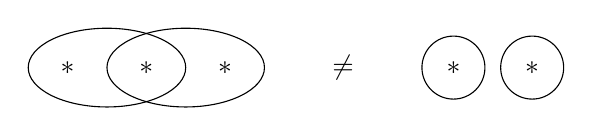
\begin{tikzpicture}
            \draw (-0.5,0) circle [x radius=1cm, y radius=0.5cm];
            \draw (0.5,0) circle [x radius=1cm, y radius=0.5cm];

            \node at (-1,0) {$\ast$};
            \node at (0,0) {$\ast$};
            \node at (1,0) {$\ast$};

            \node at (2.5,0) {$\neq$};

            \begin{scope}[xshift=4.4cm]
                \draw (-0.5,0) circle[radius=0.4cm];
                \draw (0.5,0) circle[radius=0.4cm];

                \node at (-0.5,0) {$\ast$};
                \node at (0.5,0) {$\ast$};
            \end{scope}
        \end{tikzpicture}
    \end{center}
\end{solution}

\begin{problem}
Zeigen Sie: Für alle~$n \geq 1$ gilt
\begin{equation}
    \sum_{k=1}^n k^2 = \frac{n (n+1) (2n+1)}{6}.\label{prob:eqn:sumsquare}
\end{equation}
\end{problem}

\begin{solution}
    \begin{proof}
        Wir führen eine vollständige Fallunterscheidung über~$n$ durch. Dabei ist~$A(n)$ \cref{prob:eqn:sumsquare}.

        \begin{itemize}
            \item \emph{Induktionsanfang}: Für~$n = 1$ ist $1^2 = \frac{1}{6} (1 \cdot 2 \cdot 3)$ wahr und folglich ist auch $A(1)$ wahr.
            \item \emph{Induktionsschritt}: Wenn~$A(n)$ gilt, gilt auch
                  \begin{align*}
                      \sum_{k=1}^{n+1} k^2 & = (n+1)^2 + \sum_{k=1}^n k^2 \overset{A(n)}{=} (n+1)^2 + \frac{n(n+1)(2n+1)}{6} = \frac{n+1}{6} \bigl(6(n+1) + n(2n+1)\bigr) \\
                                           & = \frac{n+1}{6} \bigl((4n+6) + n(2n+3)\bigr) = \frac{(n+1) (n+2) (2n+3)}{6},
                  \end{align*}
                  also ist auch~$A(n+1)$ wahr.\qedhere
        \end{itemize}
    \end{proof}

    Alternativ können wir das auch nicht induktiv über Teleskopsummen zeigen.

    \begin{proof}
        In der Summe heben sich der Minuend~$k^3$ des Index~$i$ mit dem Subtrahenden $-(k-1)^3$ des Index~$i+1$ auf. Damit gilt
        \begin{gather*}
            n^3 = \sum_{k=1}^n \paren*{k^3 - (k-1)^3} = 3\sum_{k=1}^n k^2 - 3\sum_{k=1}^n k + \sum_{k=1}^n 1 = 3\sum_{k=1}^n k^2 - 3\frac{n (n+1)}{2} + n \\
            \iff \sum_{k=1}^n k^2 = \frac{n^3}{3} + \frac{n^2}{2} + \frac{n}{6} = \frac{n (n+1) (2n+1)}{6}. \qedhere
        \end{gather*}
    \end{proof}
\end{solution}

\section{Körper}

Auch \emph{Rechenbereich} genannt. Körper verallgemeinern und abstrahieren die uns gewohnten rationalen oder reellen Zahlen und deren Rechenoperationen. Dennoch sollten wir uns ab sofort von den uns bekannten Beispielen lösen, da die in der (linearen) Algebra betrachteten Objekte sehr abstrakt werden und nicht unbedingt analog zu unserem Vorwissen funktionieren.

\subsection{Körperaxiome}

\begin{axiom}[Körper]
    Ein \emph{Körper} ist eine Menge~$K$ zusammen mit zwei Abbildungen
    \begin{equation*}
        +\colon K \times K \to K,\quad (a, b) \mapsto a+b \quad\qquad\text{und}\qquad\quad \cdot\colon K \times K \to K,\quad (a, b) \mapsto a\cdot b,
    \end{equation*}
    \emph{Addition} bzw.\ \emph{Multiplikation} genannt, sodass folgende Regeln (Axiome) gelten:
    \begin{enumerate}[widest=(M0), leftmargin=*]
        \refitem[(A1)] $a+(b+c) = (a+b)+c$ für alle $a, b, c \in K$ (\emph{Assoziativität der Addition});\label[axiom]{ax:field:aa}
        \refitem[(A2)] $a+b = b+a$ für alle $a, b \in K$ (\emph{Kommutativität der Addition});\label[axiom]{ax:field:ac}
        \refitem[(A3)] Es existiert ein Element $0 = 0_K \in K$ mit $a+0 = a$ für alle~$a \in K$ (Existenz eines \emph{Nullelements});\label[axiom]{ax:field:an}
        \refitem[(A4)] Zu jedem~$a \in K$ gibt es ein~$-a \in K$ mit $a+(-a) = 0$ (Existenz eines \emph{additiven Inversen});\label[axiom]{ax:field:ai}
        \refitem[(M1)] $a\cdot(b\cdot c) = (a\cdot b)\cdot c$ für alle $a, b, c \in K$ (\emph{Assoziativität der Multiplikation});\label[axiom]{ax:field:ma}
        \refitem[(M2)] $a\cdot b = b\cdot a$ für alle $a, b \in K$ (\emph{Kommutativität der Multiplikation});\label[axiom]{ax:field:mc}
        \refitem[(M3)] Es existiert ein Element $1 = 1_K \in K$ mit~$1 \neq 0$ und $1\cdot a = a$ für alle~$a \in K$ (Existenz eines \emph{Einselements});\label[axiom]{ax:field:mn}
        \refitem[(M4)] Zu jedem~$a \in K$ mit~$a \neq 0$ gibt es ein~$a^{-1} \in K$ mit~$a\cdot a^{-1} = 1$ (Existenz des \emph{multiplikativen Inversen});\label[axiom]{ax:field:mi}
        \refitem[(D)] $(a+b)\cdot c = (a\cdot c)+(b\cdot c)$ für alle $a, b, c \in K$ (\emph{Distributivität}).\label[axiom]{ax:field:d}
    \end{enumerate}
\end{axiom}

Oftmals lassen wir den Index~$K$ wie in $0_K$~und~$1_K$ weg, wenn der Kontext klar ist. Manchmal schreiben wir ihn aber hinzu, um zu verdeutlichen, dass sie zum Körper~$K$ gehören.

\begin{remark}
    Wir setzen $1 \neq 0$ voraus, d.\,h.\ ein Körper hat mindestens zwei Elemente.\footnote{Traditionell wird in der Algebra $1 \neq 0$ definiert. Es gibt aber "`esoterische"' Konzepte eines einelementigen Körpers~$\F_1$, d.\,h.\ $1 = 0$, was aber einige Körpereigenschaften verliert.}
\end{remark}

\begin{remark}
    Dabei steht der Ausdruck~$a+b$ eigentlich für~$+\bigl((a, b)\bigr)$ und~$a\cdot b$ für~$\cdot\bigl((a, b)\bigr)$. Streng genommen müssten wir z.\,B.\ Axiom~\ref{ax:field:aa} als
    \begin{equation*}
        a+(b+c) = (a+c)+b \quad\longrightarrow\quad  +\Bigl(\!\bigl(a, +\bigl((b, c)\bigr)\bigr)\!\Bigr) = +\Bigl(\!\bigl(+\bigl((a, b)\bigr), c\bigr)\!\Bigr)
    \end{equation*}
    und Axiom~\ref{ax:field:ac} als
    \begin{equation*}
        a+b = b+a \quad\longrightarrow\quad +\bigl((a, b)\bigr) = +\bigl((b, a)\bigr)
    \end{equation*}
    schreiben.
\end{remark}

\begin{notation}\label{not:field:convention}
    Neben diesen Axiomen führen wir noch einige Konventionen ein.
    \begin{itemize}
        \item Um Klammern zu sparen, gilt \emph{Punktrechnung vor Strichrechnung}. Damit können wir z.\,B.\ das Distributivgesetz~\ref{ax:field:d} umschreiben als $a\cdot c + b\cdot c$, ohne dass Verwirrung entsteht.
        \item Wir definieren $a-b \coloneqq a+(-b)$ und $ab \coloneqq a\cdot b$ für $a, b \in K$. Somit können wir Plusklammern und Malpunkte weglassen, wenn der Sinn dabei nicht verfälscht wird (z.\,B.\ nicht $1 \cdot 2 \neq 12$).
        \item Für $a, b \in K$ mit~$b \neq 0$ sei
              \begin{equation*}
                  \frac{a}{b} \coloneqq a/b \coloneqq a \cdot b^{-1}.
              \end{equation*}
    \end{itemize}
\end{notation}

Diese Regeln und Schreibweisen sind alles Konventionen und hängen nicht mit der Struktur oder den Eigenschaften eines Körper zusammen. Wir hätten genauso jede andere Konvention einführen können.

\begin{notation}
    Wir definieren kurz $K^\times \coloneqq K \setminus \mset{0}$.
\end{notation}

Ab sofort meinen wir mit~$K$ immer einen Körper mit den Operationen $+$~und~$\cdot$, falls nicht anders spezifiziert. Manchmal schreiben wir auch $(K, +, \cdot)$ für einen Körper.

\subsection{Beispiele von Körpern}

\begin{example}
    $\Q$~und~$\R$ mit den üblichen Abbildungen $+$~und~$\cdot$ sind Körper.
\end{example}

\begin{example}
    $\Z$~ist kein Körper, da (nur)~\ref{ax:field:mi} nicht erfüllt wird.
\end{example}

\begin{example}
    $\C$, die Menge der komplexen Zahlen mit $+$~und~$\cdot$ ist ein Körper.
\end{example}

\begin{example}
    Sei $K \coloneqq \mset{a, b}$ mit~$a \neq b$. Wir definieren die Abbildungen $+\colon K \times K \to K$ und $\cdot\colon K \times K \to K$ durch\footnote{Die Abbildungen ähneln der Addition und Multiplikation modulo~$2$.}
    \begin{align*}
        a + a     & = a, & a + b     & = b, & b + a     & = b, & b + b     & = a, \\
        a \cdot a & = a, & a \cdot b & = a, & b \cdot a & = a, & b \cdot b & = b.
    \end{align*}
    $K$~erfüllt alle Axiome eines Körpers, wobei das Nullelement~$0_K = a$ und das Einselement~$1_K = b$ ist, also $K = \F_2 \coloneqq \mset{0, 1}$. Der Körper ist der kleinstmögliche Körper (jeder Körper muss mindestens $0$~und~$1$ enthalten). Tatsächlich ist der Körper sogar eindeutig, was wir aber nicht beweisen werden.
\end{example}

\begin{example}
    Sei~$K \coloneqq \Q(\sqrt{2}) \coloneqq \mset{a+b\sqrt{2} \mid a, b \in \Q} \subset \R$.\footnote{Das ist eine sog.\ Körperadjunktion bzw.\ Körpererweiterung} Wir definieren die Abbildungen $+\colon K \times K \to K$ und $\cdot\colon K \times K \to K$ als Einschränkung von $+\colon \R \times \R \to \R$ und $\cdot\colon \R \times \R \to \R$ (d.\,h.\ die Abbildungen sind dieselben aus~$\R$ bis auf den kleineren Definitionsbereich). Insbesondere heißt das
    \begin{gather*}
        (a+b\sqrt{2}) + (c+d\sqrt{2}) \coloneqq (a+c) + (b+d)\sqrt{2}
        \shortintertext{und}
        (a+b\sqrt{2}) \cdot (c+d\sqrt{2}) \coloneqq (ac+2bd) + (ad+bc)\sqrt{2}.
    \end{gather*}

    Die meisten Körperaxiome sind offensichtlich erfüllt. Für~\ref{ax:field:mi} stellt sich jedoch die Frage, ob $(a+b\sqrt{2})^{-1} \in K$ für alle~$a+b\sqrt{2} \neq 0$ existiert. \emph{Antwort}: Ja, denn
    \begin{gather*}
        (a+b\sqrt{2}){-1} \coloneqq \frac{a}{a^2-2b^2} + \frac{-b}{a^2-2b^2} \sqrt{2}
        \shortintertext{mit}
        \frac{a}{a^2-2b^2} + \frac{-b}{a^2-2b^2} \sqrt{2} = \frac{a-b\sqrt{2}}{a^2-2b^2} = \frac{a-b\sqrt{2}}{(a+b\sqrt{2}) (a-b\sqrt{2})} = \frac{1}{a+b\sqrt{2}}.
    \end{gather*}

    \emph{Beachte}: Die Brüche sind definiert, weil $(a/b)^2 \neq 2 \iff a^2-2b^2 \neq 0$ wegen~$\sqrt{2} \notin \Q$.
\end{example}

\subsection{Rechenregeln in Körpern}

\begin{lemma}[Linksdistributivität]
    Es gilt $a(b+c) = ac+ac$ für alle $a, b, c \in K$.
\end{lemma}

\begin{proof}
    Es gilt $a(b+c) \overset{\text{\ref{ax:field:mc}}}{=} (b+c)a \overset{\text{\ref{ax:field:d}}}{=} ba+ca \overset{\text{\ref{ax:field:mc}}}{=} ab+ac$.
\end{proof}

\begin{lemma}[Eindeutigkeit der Null]
    Es gibt nur ein Nullelement in einem Körper.
\end{lemma}

\begin{proof}
    Seien $0'$~und~$0''$ Nullelemente im Körper~$K$. Dann gilt $0'' \overset{\text{\ref{ax:field:an}}}{=} 0''+0' \overset{\text{\ref{ax:field:ac}}}{=} 0'+0'' \overset{\text{\ref{ax:field:an}}}{=} 0'$. Dabei haben wir für die erste Gleichheit die Eigenschaft $0' = 0_K$ und für die letzte Gleichheit $0'' = 0_K$ ausgenutzt.
\end{proof}

\begin{lemma}
    Für alle~$a \in K$ gilt $0a = 0$.
\end{lemma}

\begin{proof}
    Sei~$a \in K$. Dann gelten
    \begin{gather}
        0a \overset{\text{\ref{ax:field:an}}}{=} (0+0)a \overset{\text{\ref{ax:field:d}}}{=} 0a + 0a, \label{eqn:fieldprop:timeszero}\\
        0 \overset{\text{\ref{ax:field:ai}}}{=} 0a + (-(0a)) \overset{\text{\eqref{eqn:fieldprop:timeszero}}}{=} (0a + 0a) + (-(0a)) \overset{\text{\ref{ax:field:aa}}}{=} 0a + (0a + (-(0a))) \overset{\text{\ref{ax:field:ai}}}{=} 0a + 0 \overset{\text{\ref{ax:field:an}}}{=} 0a. \tag*{\qedhere}
    \end{gather}
\end{proof}

In den Übungsaufgaben werden wir noch eine Vielzahl weiterer Regeln beweisen.

\subsection{Charakteristik eines Körpers}

\begin{notation}
    Sei $K$~ein Körper. Für~$a \in K$ und $0 \neq m \in \N$ definieren wir
    \begin{equation*}
        m \cdot a \coloneqq \underbrace{a + a + \dots + a }_\text{$m$ mal}.
    \end{equation*}
\end{notation}

\begin{definition}[Charakteristik]
    Wir definieren $\mchar(K)$ als die \emph{Charakteristik} von~$K$ als
    \begin{equation*}
        \mchar(K) \coloneqq \begin{cases}
            0                                                             & \text{falls $m \cdot 1_K \neq 0_K$ für alle $m \in \N \setminus \mset{0}$}, \\
            \min\mset{m \in \N \setminus \mset{0} \mid m \cdot 1_K = 0_K} & \text{sonst}.
        \end{cases}
    \end{equation*}
\end{definition}

\begin{lemma}\label{lem:primechar}
    Sei $K$~ein Körper mit $\mchar(K) = p > 0$. Dann ist $p$~eine Primzahl.
\end{lemma}

\begin{proof}
    Angenommen $p$~wäre keine Primzahl, sodass es $p_1, p_2 \in \N$ mit $p_1, p_2 \geq 2$ und $p = p_1p_2$ gibt. Aus der Minimalität der Charakteristik folgt $p_1 \cdot 1_K \neq 0$ und $p_2 \cdot 1_K \neq 0$. Damit gilt
    \begin{equation*}
        (p_1 \cdot 1_K) (p_2 \cdot 1_K) = (p_1p_2) \cdot 1_K = p \cdot 1_K = 0_K.
    \end{equation*}
    Aufgrund der Nullteilerfreiheit in einem Körper (s.~Übungsaufgabe) gilt $p_1 \cdot 1_K = 0_K$ oder $p_2 \cdot 1_K = 0_K$, ein Widerspruch.\footnote{Die Charakteristik hat einige interessante Eigenschaften:

        Aus einer positiven Charakteristik folgt sofort $a + a + \dots a = 0$. Sie hilft und zu bestimmen, wann ein Ausdruck null wird, was wichtig für das Rechnen im Körper ist (wir denken an $a+0 = 0$, $0a = 0$ und, dass $0^{-1}$ nicht existiert). In diesem Kontext ist $\mchar(K) = 2$ besonders wichtig, denn in dem Fall ist $a + a = 0$ für alle~$a \in K$, d.\,h.\ jedes Element ist sein eigenes additives Inverse. $\mchar(K) \neq 2$ garantiert uns die Existenz der $2 \coloneqq 1+1$.

        Jeder Teilkörper eines Körpers hat dieselbe Charakteristik wie der Körper, z.\,B.\ $\mchar(\F_2) = \mchar(\F_4) = 2$. Damit haben Körper mit gleicher Charakteristik auch eine ähnliche Struktur.

        Die Charakteristik ist eigentlich für Ringe (die später folgen) definiert. All diese Eigenschaften gelten auch für Ringe.}
\end{proof}

\lecturesep{15.~Oktober 2021}

\subsection{Die Ringe~\texorpdfstring{$\bm{\Z_m}$}{Zm}}

\begin{axiom}[Ring]
    Ein \emph{Ring} ist eine Menge~$R$ zusammen mit zwei Abbildungen
    \begin{equation*}
        +\colon R \times R \to R,\quad (a, b) \mapsto a+b \quad\qquad\text{und}\qquad\quad \cdot\colon R \times R \to R,\quad (a, b) \mapsto a \cdot b
    \end{equation*}
    \emph{Addition} bzw.\ \emph{Multiplikation} genannt, sodass folgende Regeln (Axiome) gelten:
    \begin{enumerate}[leftmargin=*, widest=(A1)]
        \refitem[(A1)] $a+(b+c) = (a+b)+c$ für alle $a, b, c \in R$ (\emph{Assoziativität der Addition});\label[axiom]{ax:ring:aa}
        \refitem[(A2)] $a+b = b+a$ für alle $a, b \in R$ (\emph{Kommutativität der Addition});\label[axiom]{ax:ring:ac}
        \refitem[(A3)] Es existiert ein Element $0 = 0_R \in R$ mit $a+0 = a$ für alle~$a \in R$ (Existenz eines \emph{Nullelements});\label[axiom]{ax:ring:an}
        \refitem[(A4)] Zu jedem~$a \in R$ gibt es ein~$-a \in R$ mit $a+(-a) = 0$ (Existenz eines \emph{additiven Inversen});\label[axiom]{ax:ring:ai}
        \refitem[(R1)] $a\cdot(b\cdot c) = (a\cdot b)\cdot c$ für alle $a, b, c \in R$ (\emph{Assoziativität der Multiplikation});\label[axiom]{ax:ring:ma}
        \refitem[(R2)] Es existiert ein Element $1 = 1_R \in R$ mit~$1 \neq 0$ und $1\cdot a = a$ für alle~$a \in R$ (Existenz eines \emph{Einselements});\label[axiom]{ax:ring:mn}
        \refitem[(D)] $(a+b)\cdot c = (a\cdot c)+(b\cdot c)$ und $a\cdot(b+c) = (a\cdot b)+(a\cdot c)$ für alle $a, b, c \in K$ (\emph{Distributivität}).\label[axiom]{ax:ring:d}
    \end{enumerate}
\end{axiom}

\begin{definition}[kommutativer Ring]
    Ein Ring~$R$ heißt \emph{kommutativ}, falls zusätzlich $a\cdot b = b\cdot a$ für alle $a, b \in \R$ gilt.
\end{definition}

\begin{remark}
    Im Vergleich zu einem Körper sind die Axiome der Addition identisch. Bei der Multiplikation fehlt lediglich die Kommutativität~\ref{ax:field:mc} und die Existenz des Inversen~\ref{ax:field:mi}. Aufgrund der fehlenden Kommutativität werden in der Distributivität beide Multiplikationsreihenfolgen angeben, die wir auch beide nachweisen müssen.
\end{remark}

\begin{remark}
    In einem Ring wird nicht verlangt, dass $1_R \neq 0_R$. Ist aber $1_R = 0_R$, so folgt daraus $a = 1_R a = 0_R a = 0_R$ für alle~$a \in R$, also $R = \mset{0_R}$.
\end{remark}

\begin{notation}[Nullring]
    Wir nennen $R = \mset{0_R}$ den trivialen\footnote{Als \emph{triviale} Objekte werden oft offensichtliche oder sehr einfache Objekte sowie uninteressante Randfälle bezeichnet.} \emph{Nullring}.
\end{notation}

Wir übernehmen für Ringe alle Schreibkonventionen in \cref{not:field:convention}, die wir für Körper festlegten (bis auf Brüche).

\begin{lemma}
    Seien $a, m \in \N$ mit~$m \geq 1$. Dann existieren eindeutig bestimmte Elemente $r, q \in \N$ mit $0 \leq r < m$, sodass $a = qm+r$ gilt. Setze $r_m(a) \coloneqq r$.
\end{lemma}

\begin{proof}
    Zu jedem~$a \in \N$ gibt es ein eindeutig bestimmtes~$q \in \N$ mit $qm \leq a < (q+1)m$. Mit $r \coloneqq a-qm$ folgt die Behauptung.
\end{proof}

\begin{definition}[$\Z$~modulo~$m$]
    Sei~$m \in \N$ mit~$m \geq 2$. Dann sei $\Z_m \coloneqq \mset{0, 1, \dots, m-1}$. Für $a, b \in \Z_m$ definieren wir noch Abbildungen $+$~und~$\cdot$ durch $a+b \coloneqq r_m(a\mathrel{+_{\,\Z}}b)$ und $a\cdot b \coloneqq r_m(a\mathrel{\cdot_{\,\Z}}b)$. (Die Operationen in den~$r_m(\dots)$ kommen aus~$\Z$.)
\end{definition}

Manchmal ist es hilfreich, auch die Operatoren aus verschiedenen Mengen durch Subskripte zu unterscheiden, also $+_K$, $\cdot_R$, etc.

\begin{lemma}
    $(\Z_m, +, \cdot)$ ist ein kommutativer Ring.\footnote{Ein sog.\ \emph{Restklassenring modulo~$m$}.}
\end{lemma}

\begin{proof}
    Übungsaufgabe.
\end{proof}

\begin{lemma}
    $(\Z_m, +, \cdot)$ ist genau dann ein Körper, wenn $m$~eine Primzahl ist.
\end{lemma}

\begin{proof}
    Angenommen $\Z_m$~ist ein Körper. Dann folgt $\mchar(\Z_m) = m$ aus der Definition der Addition über die Addition in~$\Z$ (in~$\Z$ ist $m1 = 1+1+\dots+1 = m$). Nach \cref{lem:primechar} ist $m$~eine Primzahl.

    Für die Umkehrung sei nun $m$~eine Primzahl. Zuerst zeigen wir, dass $\Z_m$ nullteilerfrei ist. Seien $a, b \in \Z_m$ mit $a\cdot b = 0 = r_m(a+b)$. Folglich wird $ab$ von~$m$ geteilt (Rest~$0$). Da $m$~eine Primzahl ist, folgt (aus dem \emph{Lemma von \textsc{Euklid}}): $m$~teilt~$a$ oder $m$~teilt~$b$. Weil nun $0 \leq a, b < m$ ist, muss $a = 0$ oder $b = 0$ sein. Folglich haben wir gezeigt, dass $\Z_m$~nullteilerfrei ist.

    Nun zeigen wir, dass jedes~$a \in \Z_m$ mit~$a \neq 0$ ein multiplikatives Inverses besitzt. Für solche~$a$ definieren wir die Abbildung $\rho_a\colon \Z_m \to \Z_m$, $x \mapsto xa$. Dann $\rho_a$~ist injektiv: Aus $xa = \rho_a(x) = \rho_a(y) = ya \iff (x-y)a = 0$ folgt aufgrund Nullteilerfreiheit $x-y = 0 \iff x = y$. Da $\Z_m$~endlich ist, ist $\rho_a$~auch surjektiv.

    Aus der Bijektion folgt, dass $0a, 1a, \dots, (m-1)a$ paarweise verschieden sind (injektiv), und diese Elemente auch jedes Element aus~$\Z_m$ repräsentiert (surjektiv), insbesondere die~$1$. Es gibt also ein~$x \in \Z_m$ mit~$xa = 1$. Zu jedem~$a \in \Z_m \setminus{0}$ gibt es also ein multiplikatives Inverses~$x \in \Z_m$, sprich $a$~ist invertierbar, was Axiom~\ref{ax:field:mi} erfüllt. Die restlichen Körperaxiome folgen aus dem kommutativen Ring.
\end{proof}

Vom kommutativen Ring zum Körper fehlt nur noch die Existenz des multiplikativen Inversen. Hierfür haben wir alle möglichen Kandidaten für das Inverse betrachtet, also $0a, 1a, \dots, (m-1)a$. Wir beobachten, dass diese Menge genau~$\Z_m$ entspricht, es also eine einfache Bijektion~$\rho_a$ geben muss, die wir auch beweisen haben. Der Trick hier war zu zeigen, dass $\Z_m$~nullteilerfrei ist (ein gutes Zeichen, da Nullteilerfreiheit eine Körpereigenschaft ist).

\begin{notation}[endlicher Körper]
    Für Primzahlen~$p$ schreiben wir auch $\F_p \coloneqq \Z_p$.
\end{notation}

\section{Vektorräume}

\emph{Vektorräume} sind wichtige Objekte, die in vielen Bereichen der Mathematik vorkommen. Das Ziel der linearen Algebra ist es, eine "`Theorie der Vektorräume"' zu entwickeln und dabei die Eigenschaften von Vektorräumen zu erforschen.

\subsection{Vektorraumaxiome}

\begin{axiom}[Vektorraum]
    Sei $K$~ein Körper.  Ein \emph{Vektorraum über~$K$} oder \emph{$K$"~Vektorraum} ist eine Menge~$V$ zusammen mit zwei Abbildungen
    \begin{equation*}
        +\colon V \times V \to V,\quad (v_1, v_2) \mapsto v_1+v_2 \quad\qquad\text{und}\qquad\quad \cdot\colon K \times V \to V,\quad (a, v) \mapsto a\cdot v,
    \end{equation*}
    \emph{Addition} bzw.\ \emph{Skalarmultiplikation} genannt, sodass folgende Regeln (Axiome) gelten:
    \begin{enumerate}[leftmargin=*, widest=(SM0)]
        \refitem[(A1)] $v_1+(v_2+v_3) = (v_1+v_2)+v_3$ für alle $v_1, v_2, v_3 \in V$ (\emph{Assoziativität der Addition});\label[axiom]{ax:vecspace:aa}
        \refitem[(A2)] $v_1+v_2 = v_2+v_1$ für alle $v_1, v_2 \in V$ (\emph{Kommutativität der Addition});\label[axiom]{ax:vecspace:ac}
        \refitem[(A3)] Es existiert ein Element $0 = 0_V \in V$ mit $v + 0_V = v$ für alle~$v \in V$ (Existenz eines \emph{Nullelements});\label[axiom]{ax:vecspace:an}
        \refitem[(A4)] Zu jedem~$v \in V$ gibt es ein~$-v \in V$ mit $v+(-v) = 0$ (Existenz eines \emph{additiven Inversen});\label[axiom]{ax:vecspace:ai}
        \refitem[(SM1)] $(ab)\cdot v = a\cdot(b\cdot v)$ für alle $a, b \in K$ und~$v \in V$;\label[axiom]{ax:vecspace:smcomp}
        \refitem[(SM2)] $1_K \cdot v = v$ für alle~$v \in V$;\label[axiom]{ax:vecspace:smn}
        \refitem[(SM3)] $a\cdot(v_1+v_2) = a\cdot v_1 + a\cdot v_2$ für alle~$a \in K$ und $v_1, v_2 \in V$;\label[axiom]{ax:vecspace:smdv}
        \refitem[(SM4)] $(a+b)\cdot v = (a\cdot v)+(b\cdot v)$ für alle~$a, b \in K$ und~$v \in V$.\label[axiom]{ax:vecspace:smdf}
    \end{enumerate}
\end{axiom}

Wir schreiben oft auch einfach~$V$ für den $K$"~Vektorraum $(V,+,\cdot)$.

\begin{notation}
    Um die Notation zu vereinfachen, legen wir $v_1-v_2 \coloneqq v_1+(-v_2)$, $av \coloneqq a \cdot v$ für alle $v_1, v_2, v \in V$ und $a \in K$ sowie \emph{Punkt"~ vor Strichrechnung} fest.
\end{notation}

\begin{notation}[Vektor, Skalar, Nullvektor]
    Die Elemente von~$V$ nennen wir \emph{Vektoren}, die Elemente von~$K$ nennen wir \emph{Skalare}. Das Nullelement~$0_V$ heißt \emph{Nullvektor} oder auch \emph{die Null von~$V$}.
\end{notation}

\begin{remark}
    Es ist sehr wichtig, zu wissen, welchen Grundkörper~$K$ der Vektorraum hat. Dieselbe Menge~$V$, aber über zwei verschiedene Körper $K_1$~und~$K_2$, sind zwei verschiedene Vektorräume, nämlich ein $K_1$"~ und ein $K_2$"~Vektorraum. Im Allgemeinen ist ein Vektorraum über einen anderen Körper kein Vektorraum mehr, da er z.\,B.\ nicht mehr abgeschlossen ist.
\end{remark}

\begin{remark}
    Die Skalarmultiplikation multipliziert ein Skalar mit einem Vektor (wie der Name schon sagt, also \underline{kein} Skalarprodukt). Wir beachten auch die Reihenfolge der Skalarmultiplikation, d.\,h.\ Skalare werden von \emph{links} multipliziert.
\end{remark}

Wie bei Körpern gibt es eine Vielzahl an Rechenregeln für Vektorräume, die wir in den Übungen beweisen.

\subsection{Beispiele von Vektorräumen}

\begin{notation}[Nullvektorraum]
    Sei $V \coloneqq \mset{0}$ über~$K$ der (triviale) \emph{Nullvektorraum} (oft auch einfach nur $V = 0$). Addition und Skalarmultiplikation können nur auf genau eine Weise definiert werden:
    \begin{gather*}
        +\colon V\times V \to V,\qquad 0+0 \mapsto 0 \\
        \cdot\colon V\times V \to V,\qquad 0\cdot0 \mapsto 0 \\
    \end{gather*}
\end{notation}

\begin{example}
    Sei $K$~ein Körper. Dann ist $K$ ein $K$"~Vektorraum mit Addition und Skalarmultiplikation definiert als Addition und Multiplikation von~$K$.
\end{example}

\begin{definition}[Standardvektorraum]
    Sei $K$~ein Körper. Für~$n \geq 1$ sei $V \coloneqq K^n$ das $n$"~fache kartesische Produkt von~$K$. Die Elemente aus~$K^n$ schreiben wir oft als Spalten
    \begin{equation*}
        \p{a_1\\\vdots\\a_n}
    \end{equation*}
    mit $a_1,\dots,a_n \in K$. Wir definieren komponentenweise
    \begin{gather*}
        +\colon V\times V \to V \quad\text{durch}\quad \paren*{\p{a_1\\\vdots\\a_n}, \p{b_1\\\vdots\\b_n}} \mapsto \p{a_1+b_1\\\vdots\\a_n+b_n}
        \shortintertext{und}
        \cdot\colon K\times V \to V \quad\text{durch}\quad \paren*{a, \p{b_1\\\vdots\\b_n}} \mapsto \p{ab_1\\\vdots\\ab_n}.
    \end{gather*}

    Dann ist $(V,+,\cdot)$ ein $K$"~Vektorraum, der sog.\ \emph{Standardvektorraum}. Wir legen $K^0 \coloneqq 0$ aus~$K$ fest.

    Dabei stammt die komponentenweise Addition und Multiplikation aus~$K$.
\end{definition}

In~$V = \R^2$ mit~$K = \R$ können wir Addition und Skalarmultiplikation visualisieren, indem wir Vektoren als Pfeile darstellen. Addition heißt dann Aneinanderreihen von Pfeilen; Skalarmultiplikation heißt dann Strecken\slash Stauchen oder Änderung der Richtung von Pfeilen. Das sollte aus der Schule bekannt sein.
\begin{center}
    \begin{tikzpicture}
        \draw[->] (-2.5,0) -- (5,0) node[below] {$\R$};
        \draw[->] (0,-1.5) -- (0,2.5) node[left] {$\R$};
        \draw[->] (0,0) -- (-2,1) node[left] {$v$};
        \draw[->] (0,0) -- (2,-1) node[below left] {$-v$};
        \draw[->] (0,0) -- (3,1) node[below right] {$w$};
        \draw[->] (0,0) -- (4.5,1.5) node[below right] {$\frac{3}{2}w$};
        \draw[->] (0,0) -- (1,2) node[above] {$v+w$};
        \draw[dashed] (-2,1) -- (1,2) -- (3,1);
    \end{tikzpicture}
\end{center}

Ein sehr wichtiges Beispiel von Vektorräumen:

\begin{definition}[Funktionenraum]
    Sei $K$~ein Körper und sei $I \neq \varnothing$ eine Menge. Wir setzen $V \coloneqq K^I \coloneqq \map(I, K)$ und definieren
    \begin{gather*}
        +\colon V \times V \to V,\quad (f,g) \mapsto f+g \quad\qquad\text{und}\qquad\quad \cdot\colon K \times V \to V,\quad (a,f) \mapsto af,
        \shortintertext{punktweise durch}
        (f+g)(x) \coloneqq f(x)+g(x) \quad\qquad\text{und}\qquad\quad (af)(x) \coloneqq a(f(x))
    \end{gather*}
    für alle $f,g \in V$, $a \in K$, und $x \in I$.

    Dann ist $(V,+,\cdot)$ ein $K$"~Vektorraum, der sog.\ \emph{(lineare) Funktionenraum}. Wir definieren $K^\varnothing = 0$ als Nullabbildung.
\end{definition}

Dabei ist in den Definitionsgleichungen auf der linken Seite Addition und Skalarmultiplikation in~$V$, sowie auf der rechten Seite Addition und Multiplikation in~$K$.\footnote{An dieser Stelle fragt man sich vielleicht, warum der Standardvektorraum~$K^n$ und der Funktionenraum~$K^I$ identisch notiert werden. Das liegt daran, dass sie tatsächlich "`identisch"' (d.\,h.\ \emph{isomorph}) sind, weil es eine Bijektion wie in \cref{ex:map:setisoproduct} gibt.}\textsuperscript{,}\footnote{Für~$I = \N$ lässt sich auch der "`unendlichdimensionale"' \emph{Folgenraum}
    \begin{equation*}
        K^\N \coloneqq \mset{(a_1,a_2,a_3,\dots) \mid a_i \in K \text{ für alle } i \in \N}
    \end{equation*}
    (wie in der Analysis) definieren.}

Ein noch wichtigeres Beispiel ist

\begin{definition}
    Sei $K$~ein Körper und sei $I \neq \varnothing$ eine Menge. Dann ist
    \begin{equation*}
        K^{(I)} \coloneqq \mset{f \in K^I \mid f(x) \neq 0 \text{ für nur endlich viele } x \in I}
    \end{equation*}
    ein $K$"~Vektorraum, wobei wir Addition und Skalarmultiplikation von~$K^I$ benutzen. Wir definieren $K^{(\varnothing)} = 0$ als Nullabbildung.
\end{definition}

Jede Abbildung $f \in K^{(I)}$ bildet also fast alle~$x \in I$ (bis auf endlich viele) auf~$0$ ab.

\begin{definition}[Teilkörper]
    Sei $(L,+,\cdot)$ ein Körper und sei $K$~eine Teilmenge von~$L$, sodass die Eigenschaften
    \begin{enumerate}
        \item $0, 1 \in K$ (neutrale Elemente);
        \item $a+b \in K$ für alle $a,b \in K$ (Abgeschlossenheit unter Addition);\label{def:subfield:add}
        \item $a\cdot b \in K$ für alle $a,b \in K$ (Abgeschlossenheit unter Multiplikation);\label{def:subfield:mul}
        \item $-a \in K$ für alle~$a \in K$ (additive Inverse) und
        \item $a^{-1} \in K$ für alle~$a \in K^\times$ (multiplikative Inverse)
    \end{enumerate}
    erfüllt sind. Durch Einschränkung erhalten wir die Abbildungen
    \begin{equation*}
        +\colon K\times K \to K \quad\qquad\text{und}\qquad\quad \cdot\colon K\times K \to K.
    \end{equation*}
    (Das ist aufgrund der Abgeschlossenheit von $+$~und~$\cdot$ garantiert, s.~\cref{def:subfield:add,def:subfield:mul}.) Wir können leicht überprüfen, dass $K$~einen Körper bildet, und nennen~$K$ einen \emph{Teilkörper} von~$L$.
\end{definition}

\begin{example}
    Ist $K$~ein Teilkörper von~$L$, so ist $L$~ein $K$"~Vektorraum, wobei die Skalarmultiplikation $\cdot\colon K\times L \to L$ durch Einschränkung der Multiplikation $\dot\colon L\times L \to L$ definiert ist.

    Bspw.\ ist der Körper~$\Q(\sqrt{2})$ ein $\Q$"~Vektorraum und $\R$~sowohl ein~$\Q$"~ als auch ein $\Q(\sqrt{2})$"~Vektorraum.
\end{example}

\begin{definition}[externe direkte Summe]
    Seien $V$~und~$W$ zwei $K$"~Vektorräume. Dann ist die $V \times W$ wieder ein $K$"~Vektorraum, wobei Addition und Skalarmultiplikation komponentenweise definiert sind durch
    \begin{gather*}
        (v_1,w_1) + (v_2,w_2) \coloneqq (v_1+v_2, w_1+w_2) \qquad\text{und}\qquad a(v,w) \coloneqq (av, aw)
    \end{gather*}
    für alle $v,v_1,v_2 \in V$, $w,w_1,w_2 \in W$ und $a \in K$. Der $K$"~Vektorraum $V \times W$ nennen wir die \emph{(externe) direkte Summe} von $V$~und~$W$ und schreiben $V \oplus W$.
\end{definition}

Noch ein Beispiel aus der Analysis.

\begin{example}
    Sei $I = [a,b]$ ein abgeschlossenes Intervall in~$\R$ und sei
    \begin{equation*}
        C^0(I) \coloneqq \mset{\text{stetige Funktionen } I \to \R}
    \end{equation*}
    eine Teilmenge von~$\R^I$. Dann ist $C^0(I)$~ein $\R$"~Vektorraum mit der Einschränkung von $+\colon \R^I\times\R^I \to \R^I$ und $\cdot\colon \R\times\R^I \to \R^I$ auf die neue Definitionsmenge~$I \subset \R$.
\end{example}

\lecturesep{19.~Oktober 2021}

\subsection{Unterräume}

\begin{definition}
    Sei $V$~ein $K$"~Vektorraum. Eine Teilmenge~$U$ von~$V$ heißt \emph{Unterraum} von~$V$, falls gilt:
    \begin{enumerate}
        \item $U \neq \varnothing$;
        \item $u_1+u_2 \in U$ für alle $u_1,u_2 \in U$ (\emph{Abgeschlossenheit bzgl.\ Addition}) und\label{def:subspace:add}
        \item $au \in U$ für alle~$a \in K$ und~$u \in U$ (\emph{Abgeschlossenheit bzgl.\ Skalarmultiplikation}).\label{def:subspace:mul}
    \end{enumerate}
\end{definition}

\begin{lemma}
    Sei $U$~ein Unterraum von~$V$. Durch Einschränkung der Addition und Skalarmultiplikation von~$V$ erhalten wir Abbildungen $+\colon U\times U \to U$ und $\cdot\colon K\times U \to U$ (was aufgrund \cref{def:subfield:add,def:subfield:mul} möglich ist). Dann ist $U$ zusammen mit beiden Einschränkungen wieder ein $K$"~Vektorraum.
\end{lemma}

\begin{proof}
    Sei~$u \in U$. Aus \cref{def:subfield:mul} folgen $0u = 0 \in U$ und $(-1)u = -u \in U$. Deshalb gelten die Axiome \ref{ax:vecspace:an}~und~\ref{ax:vecspace:ai}. Alle anderen Axiome folgen aus~$V$.
\end{proof}

\begin{example}
    Die Teilmengen~$V$ und~$\mset{0}$ (statt~$\mset{0}$ schreiben wir oft nur~$0$) sind Unterräume von~$V$, die sog.\ \emph{trivialen Unterräume}.
\end{example}

\begin{example}
    Sei~$v \in V$. Dann ist
    \begin{equation*}
        U_v \coloneqq Kv \coloneqq \mset{av \mid a \in K}
    \end{equation*}
    der kleinste Unterraum\footnote{An der Stelle müssten wir definieren, was "`klein"' i.\,S.\,v.\ Unterräumen bedeuten soll. Hier meint der Dozent wahrscheinlich die \emph{Dimension}, die später drankommt.} von~$V$, welcher $v$~enthält.
\end{example}

\begin{definition}[Gerade]
    Ist~$v \neq 0$, so nennen wir
    \begin{equation*}
        U_v \coloneqq Kv \coloneqq \mset{av \mid a \in K}
    \end{equation*}
    die durch~$v$ verlaufende \emph{Gerade}.
\end{definition}

\begin{example}
    Für jede Menge~$I$ ist $K^{(I)}$~ein Unterraum von~$K^I$, denn nach Addition und Skalarmultiplikation hat jede Abbildung immer noch nur endlich viele Stellen ungleich~$0$.
\end{example}

\begin{example}
    Sei $I = [a,b]$ ein Intervall in~$\R$. Dann ist $C^0(I)$~ein Unterraum von~$\R^I$, weil sich die Stetigkeit unter Addition und Skalarmultiplikation nicht ändert.
\end{example}

\begin{example}
    Die Elemente des $\R$"~Vektorraums~$\R^\N$ sind die in der Analysis behandelten reellen Folgen. Die Teilmenge der konvergenten reellen Folgen ist ein Unterraum von~$\R^\N$, da aufgrund der Grenzwertsätze die Folgen nach Addition und Skalarmultiplikation immer noch konvergieren.
\end{example}

\begin{example}
    Sei~$a \in K$. Wir definieren
    \begin{equation*}
        U(a) \coloneqq \mset*{\p{a\\b} \mmid b \in K}.
    \end{equation*}
    Dann ist $U(a)$ genau dann ein Unterraum von~$K^2$, wenn $a = 0$.
\end{example}

\begin{definition}[Durchschnitt, Summe]
    Seien $U_1$~und~$U_2$ Unterräume von~$V$. Dann ist $U_1 \cap U_2$ der \emph{Durchschnitt} von $U_1$~und~$U_2$ sowie
    \begin{equation*}
        U_1+U_2 \coloneqq \mset{u_1+u_2 \mid u_1 \in U_1, u_2 \in U_2}
    \end{equation*}
    die \emph{Summe} von $U_1$~und~$U_2$.
\end{definition}

\begin{lemma}
    $U_1 \cap U_2$ und $U_1+U_2$ sind Unterräume von~$V$.
\end{lemma}

\begin{definition}[interne direkte Summe]
    Seien $U_1$~und~$U_2$ Unterräume von~$V$. Ist $U_1 \cap U_2 = 0$, so nennen wir
    \begin{equation*}
        U_1\oplus U_2 \coloneqq U_1+U_2
    \end{equation*}
    die \emph{(interne) direkte Summe} von $U_1$~und~$U_2$.
\end{definition}

\begin{definition}[Summe, interne direkte Summe von Familien]
    Sei $I$~eine Indexmenge, und für jedes~$i \in I$ sei $U_i$~ein Unterraum von~$V$ (kurz $(U_i)_{i\in I}$ eine Familie von Unterräumen von~$V$). Die \emph{Summe}
    \begin{equation*}
        \sum_{i\in I} U_i
    \end{equation*}
    der Unterräume~$U_i$ ist die Menge aller Vektoren~$v \in V$, für die es eine endliche Teilmenge~$J \subseteq I$ gibt, sodass
    \begin{equation*}
        v = \sum_{j\in J} u_j \qquad\text{mit } u_j \in U_j \text{ für alle } j \in J.
    \end{equation*}

    Ist
    \begin{equation*}
        U_j \cap \paren*{\sum_{i\in I\setminus{j}} U_i} = 0 \qquad\text{für alle } j \in I,
    \end{equation*}
    so nennen wir die Summe \emph{(interne) direkte Summe} und schreiben
    \begin{equation*}
        \bigoplus_{i\in I} U_i \coloneqq \sum_{i\in I} U_i.
    \end{equation*}
\end{definition}

Jedes $v \in (U_i)_{i\in I}$ ist also eine Summe von endlich vielen Vektoren~$u_j$, wobei jedes~$u_j$ von einem anderen Unterraum kommt.\footnote{Anders formuliert: Jeder Vektor~$v$ der internen Summe ist die Summe $\sum_{i\in I} u_i$ mit $u_i \in U_i$, wobei $u_i \neq 0$ nur für endlich viele~$u_i$ gilt. Vgl.\ mit der Definition von~$K^{(I)}$.}\textsuperscript{,}\footnote{Eine witzige Eigenschaft: Für zwei Untervektorräume $U$~und~$W$ von~$V$ gilt
    \begin{equation*}
        U\times\mset{0} \oplus \mset{0}\times W = U \oplus W,
    \end{equation*}
    also $(u, 0) + (0,w) = (u,w)$, wobei auf der linken Seite die \emph{interne} direkte Summe und auf der rechten Seite die \emph{externe} direkte Summe gemeint ist. Die Vektorräume auf der linken Seite teilen sich nur den Vektor $(0, 0)$.}

\begin{lemma}
    $\bigcup_{i\in I} U_i$ und $\sum_{i\in I} U_i$ sind Unterräume von~$V$.
\end{lemma}

Betrachten wir Standardvektorräume (wie z.\,B.~$\R^2$), dann können wir uns Untervektorräume als z.\,B.\ den Ursprung, Geraden, Ebenen, Räume, etc.\ vorstellen, die den Ursprung enthalten. Insbesondere sind $U_v$~Ursprungsgeraden. Die interne Summe zweier verschiedener Geraden in~$\R^2$ ist~$\R^2$ selbst; die Summe ist auch direkt, da sie nur~$0$ teilen.

\section{Lineare Abbildungen}

Die "`Theorie der Vektorräume"' wird interessant, wenn wir noch Abbildungen zwischen Vektorräumen betrachten. Dabei sollen sie die Vektorraumstruktur\footnote{Wichtig ist, dass die hier betrachteten Homomorphismen \emph{Vektorraumstrukturen erhalten}, d.\,h.\ sie sind mit der Vektorraumstruktur \emph{verträglich}. Es gibt noch viele andere Homomorphismen, wie z.\,B.\ Mengenhomomorphismen (das sind die Abbildungen), Gruppenhomomorphismen, Homomorphismen zwischen topologischen Räumen (sog.\ Homöomorphismen), etc.} erhalten, d.\,h.\ mit der Addition und Skalarmultiplikation innerhalb des Start"~ und Zielvektorraums kompatibel sein. Das führt zu \emph{linearen Abbildungen} bzw.\ \emph{Homomorphismen} ("`Gleich-Gestalter"'). Das vorläufige Ziel wird es sein, lineare Abbildungen zu verstehen.

\subsection{Definition}

\begin{definition}[lineare Abbildung]
    Seien $V$~und~$W$ zwei $K$"~Vektorräume. Eine Abbildung $f\colon V \to W$ heißt \emph{linear} (oder \emph{$K$"~linear}), falls folgende Bedingungen gelten:
    \begin{enumerate}
        \item $f(v_1+v_2) = f(v_1)+f(v_2)$ für alle $v_1,v_2 \in V$; und
        \item $f(av) = af(v)$ für alle~$v \in V$ und~$a \in K$.
    \end{enumerate}
\end{definition}

Dabei finden Addition und Skalarmultiplikation zwischen den Argumenten der Abbildung in~$V$ und zwischen den Bildern der Abbildung in~$W$ statt. Anders geschrieben:
\begin{align*}
    f(v_1\mathrel{+_V}v_2) & = f(v_1)\mathrel{+_W}f(v_2), \\
    f(a\mathrel{\cdot_V}v) & = a\mathrel{\cdot_W}f(v)
\end{align*}

\begin{definition}[Homomorphismus, Endomorphismus]
    Ist~$f\colon V \to W$ linear, so nennen wir~$f$ einen \emph{Homomorphismus}. Ist zudem $V = W$, so nennen wir~$f$ einen \emph{Endomorphismus} (also $f\colon V \to V$).

    Weiterhin definieren wir
    \begin{gather*}
        \hom(V,W) \coloneqq \mset{f \in \map(V,W) \mid f \text{ ist ein Homomorphismus}}
        \shortintertext{und}
        \mend(V) \coloneqq \hom(V,V).
    \end{gather*}
\end{definition}

\begin{definition}[Monomorphismus, Epimorphismus, Isomorphismus]
    Sei $f\colon V \to W$ ein Homomorphismus.
    \begin{itemize}
        \item $f$~ist ein \emph{Monomorphismus}, falls $f$~injektiv ist.
        \item $f$~ist ein \emph{Epimorphismus}, falls $f$~surjektiv ist.
        \item $f$~ist ein \emph{Isomorphismus}, falls $f$~bijektiv ist.
    \end{itemize}
\end{definition}

\begin{definition}[isomorph]
    Zwei $K$~Vektorräume $V$~und~$W$ heißen \emph{isomorph}, falls ein Isomorphismus $f\colon V \to W$ existiert. Wir schreiben dann $V \cong W$.
\end{definition}

Der Begriff der Isomorphie ist sehr mächtig, da er uns erlaubt, innerhalb der linearen Algebra die beiden Objekte "`gleichzusetzen"', d.\,h.\ die Objekte sind zueinander äquivalent und verhalten sich auch (unter Addition und Skalarmultiplikation) gleich.\footnote{Zusätzlich definiert man einen \emph{Automorphismus} als einen bijektiven Endomorphismus, also Isomorphismus und Endomorphismus gleichzeitig.}

\begin{lemma}\label{lem:hom:def}
    Seien $V$~und~$W$ zwei $K$"~Vektorräume. Eine Abbildung $f\colon V \to w$ ist genau dann linear, wenn
    \begin{equation*}
        f(a_1v_1 + a_2v_2) = a_1f(v_1) + a_2f(v_2)
    \end{equation*}
    für alle $a_1,a_2 \in K$ und $v_1,v_2 \in V$ gilt.
\end{lemma}

\begin{proof}
    Übungsaufgabe.
\end{proof}

\subsection{Beispiele von linearen Abbildungen}

\begin{definition}[Nullabbildung]
    Seien $V$~und~$W$ zwei $K$"~Vektorräume. Die \emph{Nullabbildung}
    \begin{equation*}
        f\colon V \to W,\quad v \mapsto 0 \quad\text{für alle } v \in V
    \end{equation*}
    ist ein Homomorphismus. Wir schreiben $f = 0$.
\end{definition}

\begin{definition}[Identität]
    Sei $V$~ein $K$"~Vektorraum. Die \emph{Identität}
    \begin{equation*}
        f\colon V \to V,\quad v \mapsto v \quad\text{ für alle } v \in V
    \end{equation*}
    ist ein Homomorphismus. Wir schreiben $f = \id_V$.
\end{definition}

Die Identität ist ein bijektiver Endomorphismus, also ein Isomorphismus und insbesondere ein Homomorphismus.

\begin{example}\leavevmode
    \begin{enumerate}
        \item Sei $V$~ein $K$"~Vektorraum und sei~$a \in K$. Die Abbildung $f_a\colon V \to V$, $v \mapsto av$ für alle~$v \in V$ ist ein Homomorphismus. Ist $a \neq 0$, d.\,h.\ $f_a \neq 0$, so ist $f_a$~sogar ein Isomorphismus.
        \item Für jeden Homomorphismus $f\colon K \to K$ gibt es ein~$a \in K$ mit~$f = f_a$. Für alle~$\lambda \in K$ gilt nämlich $f(\lambda) = f(\lambda1) = \lambda f(1)$. Dann können wir $a \coloneqq f(1)$ setzen.
        \item Die Graphen der Homomorphismen $f\colon K \to K$ sind genau die Geraden~$U_v \subseteq K^2$, wobei $v = (a,b)$ mit~$a \neq 0$ ist. Die Punkte des Graphen sind nämlich $(\lambda,f(\lambda)) = (\lambda,\lambda f(1)) = \lambda(1,f(1))$ für alle~$\lambda \in K$. Für~$a = 0$ wäre $f$~nur auf~$0$ definiert.
    \end{enumerate}
\end{example}

\begin{example}\label{ex:hom:matrixvector}
    Sei $K$~ein Körper und sei $(a,b,c,d) \in K^4$ gegeben. Die Abbildung\footnote{Das ist das Matrix-Vektor-Produkt.}
    \begin{equation*}
        f\colon K^2 \to K^2,\quad \p{x\\y} \mapsto \p{ax+by\\cx+dy}
    \end{equation*}
    ist ein Homomorphismus.

    (Um das nachzuweisen, setzen wir einfach in die Definition linearer Abbildungen ein. Für die Addition gilt
    \begin{equation*}
        f\paren*{\p{x_1\\y_1} + \p{x_2\\y_2}} = \p{a(x_1+x_2) + b(y_1+y_2) \\ c(x_1+x_2) + d(y_1+y_2)} = \p{ax_1+by_1\\cx_1+dy_1} + \p{ax_2+by_2\\cx_2+dy_2} = f\paren*{\p{x_1\\y_1}} + f\paren*{\p{x_2\\y_2}}.
    \end{equation*}
    Analog können wir zeigen, dass die Abbildung mit der Skalarmultiplikation kompatibel ist.)
\end{example}

\begin{example}
    Die Abbildung $f\colon \R \to \R$, $x \mapsto x^2$ ist kein Homomorphismus bzw.\ nicht $\R$"~linear, denn z.\,B.\ gilt $16 = f(2+2) \neq f(2)+f(2) = 8$.
\end{example}

\emph{Warnung}: In der linearen Algebra gibt es viele verschiedene Nullen. Z.\,B.\ seien $V$~und~$W$ zwei $K$"~Vektorräume. $0$~kann nun die Null~$0_K$ in~$K$, die Null~$0_V$ in~$V$, die Null~$0_W$ in~$W$, die Nullabbildung $0\colon V \to W$ oder der triviale Unterraum~$\mset{0}$ sein.

\subsection{Erste Eigenschaften linearer Abbildungen}

Für das restliche Kapitel seien $V$~und~$W$ zwei $K$"~Vektorräume.

\begin{lemma}
    Sei $f\colon V \to W$ ein Homomorphismus. Dann gilt $f(0) = 0$.
\end{lemma}

\begin{proof}
    Es gibt zwei Möglichkeiten, die Aussage zu beweisen.

    Erster Beweis: Es gilt
    \begin{equation*}
        f(0) \overset{\ref{ax:vecspace:an}}{=} f(0+0) \overset{\text{Hom.}}{=} f(0)+f(0).
    \end{equation*}
    Daraus folgt
    \begin{equation*}
        0 \overset{\ref{ax:vecspace:ai}}{=} f(0)-f(0) = (f(0)+f(0)) - f(0) \overset{\ref{ax:vecspace:aa}}{=} f(0) + (f(0)-f(0)) \overset{\ref{ax:vecspace:ai}}{=} f(0)+0 \overset{\ref{ax:vecspace:an}}{=} f(0).
    \end{equation*}

    Zweiter Beweis: Für die Nullen $0_K \in K$, $0_V \in V$ und~$0_W \in W$ gilt mit der Rechenregel $0v = 0$
    \begin{equation*}
        f(0_V) = f(0_K0_V) \overset{\text{Hom.}}{=} 0_Kf(0_V) = 0_W. \qedhere
    \end{equation*}
\end{proof}

Der zweite Beweis ist zwar kürzer, ist aber weniger elementar.

\begin{lemma}
    Sei $f\colon V \to W$ ein Isomorphismus. Dann ist die Umkehrabbildung $f^{-1}\colon W \to V$ wieder ein Isomorphismus.
\end{lemma}

\begin{proof}
    Aus den Eigenschaften von Bijektionen wissen wir, dass~$f^{-1}$ existiert und auch bijektiv ist. Wir müssen noch zeigen, dass $f^{-1}$~linear ist.

    Weil $f$~bijektiv ist, ist jedes~$w \in W$ von der Form~$f(v) = w$ für ein eindeutig bestimmtes~$v \in V$. Dann gelten für alle $v,v_1,v_2 \in V$ und~$a \in K$
    \begin{gather*}
        f^{-1}(f(v_1) + f(v_2)) = f^{-1}(f(v_1+v_2)) = v_1+v_2 = f^{-1}(f(v_1)) + f^{-1}(f(v_2))
        \shortintertext{und}
        f^{-1}(a(f(v))) = f^{-1}(f(av)) = av = af^{-1}(f(v)).
    \end{gather*}
    Folglich ist $f^{-1}$~linear.
\end{proof}

\begin{lemma}
    Seien $f\colon U \to V$ und $g\colon V \to W$ Homomorphismen. Dann ist die Komposition $g\circ f\colon U \to W$ auch ein Homomorphismus.
\end{lemma}

\begin{proof}
    Wir verwenden \cref{lem:hom:def}. Für alle $a_1,a_2 \in K$ und $v_1,v_2 \in V$ gilt
    \begin{align*}
        (g\circ f)(a_1u_2 + a_2u_2) & = g(f(a_1u_1 + a_2u_2)) \overset{\text{Hom.~$f$}}{=} g(a_1f(u_1) + a_2f(u_2))       \\
        \overset{\text{Hom.~$g$}}   & {=} a_1g(f(u_1)) + a_2g(f(u_2)) = a_1(g\circ f)(u_1) + a_2(g\circ f)(u_2). \qedhere
    \end{align*}
\end{proof}

\lecturesep{22.~Oktober 2021}

\begin{lemma}
    Für alle $f,g \in \hom(V,W)$ und~$a \in K$ definieren wir Abbildungen (Addition und Skalarmultiplikation eines Funktionenraums)
    \begin{equation*}
        f+g\colon V \to W,\quad v \mapsto f(v)+g(v) \qquad\text{und}\qquad af\colon V \to W,\quad v \mapsto a(f(v)).
    \end{equation*}
    Dann ist $(\hom(V,W),+,\cdot)$ ein $K$"~Vektorraum
\end{lemma}

\begin{proof}\leavevmode
    \begin{itemize}
        \item Zuerst müssen wir zeigen, dass die Addition und Skalarmultiplikation auf $\hom(V,W)$ abgeschlossen ist, d.\,h., dass $f+g$ und~$af$ linear sind. Dafür können wir leicht überprüfen, dass
              \begin{equation*}
                  (f+g)(\lambda_1v_1+\lambda_2v_2) = \lambda_1(f+g)(v_1)+\lambda_2(f+g)(v_2)
              \end{equation*}
              für alle $v_1,v_2 \in V$ und $\lambda_1,\lambda_2 \in K$ gilt.
        \item Die Axiome \ref{ax:vecspace:aa}~und~\ref{ax:vecspace:ac} in $\hom(V,W)$ folgen aus den Axiomen \ref{ax:vecspace:aa}~und~\ref{ax:vecspace:ac} in~$W$.
        \item Der Nullvektor in $\hom(V,W)$ (Axiom~\ref{ax:vecspace:an}) ist die Nullabbildung $0\colon V \to W$, ein Homomorphismus.
        \item Für jedes $f \in \hom(V,W)$ definieren wir $-f\colon V \to W$, $v \mapsto -(f(v))$ als das additive Inverse. Wir sehen leicht, dass $-f \in \hom(V,W)$. Dann gilt
              \begin{equation*}
                  (f+(-f))(v) = f(v)+(-(f(v))) = 0 \qquad\text{für alle } v \in V.
              \end{equation*}
              Also gilt Axiom~\ref{ax:vecspace:ai} in $\hom(V,W)$.
        \item Für alle $f,g \in \hom(V,W)$, $a \in K$ und~$v \in V$ gilt
              \begin{align*}
                  (a(f+g))(v) & = a((f+g)(v)) = a(f(v)+g(v)) \underset{\text{in }W}{\overset{\ref{ax:vecspace:smdv}}{=}} a(f(v))+a(g(v)) \\
                              & = (af)(v)+(ag)(v) = (af+ag)(v).
              \end{align*}
              Also gilt Axiom~\ref{ax:vecspace:smdv} in $\hom(V,W)$.
        \item Den Nachweis der Axiome \ref{ax:vecspace:smcomp},~\ref{ax:vecspace:smn} und~\ref{ax:vecspace:smdf} können wir ähnlich führen.\qedhere
    \end{itemize}
\end{proof}

\begin{lemma}\label{lem:hom:id}
    Sei $f\colon V \to W$ ein Homomorphismus.
    \begin{enumerate}
        \item Existiert ein Homomorphismus $g\colon W \to V$ mit $g\circ f = \id_V$, so ist $f$~ein Monomorphismus.
        \item Existiert ein Homomorphismus $g\colon W \to V$ mit $f\circ g = \id_W$, so ist $f$~ein Epimorphismus.
    \end{enumerate}
\end{lemma}

\begin{proof}
    Übungsaufgabe.
\end{proof}

\begin{remark}
    Die Umkehrung der beiden Aussagen in \cref{lem:hom:id} gilt auch. Der Beweis dazu erfolgt später.\footnote{Wir werden sehen, dass das mit der Invertierbarkeit von Matrizen zu tun hat, wobei $g$~ein Produkt von Elementarmatrizen ist.}
\end{remark}

\subsection{Lineare Abbildungen und affine Geraden}

\begin{definition}[Restklasse modulo~$U$]
    Sei $V$~ein $K$"~Vektorraum und sei $U$~ein Unterraum von~$V$ sowie~$v \in V$. Dann ist die \emph{Restklasse von~$v$ modulo~$U$} definiert als die Menge
    \begin{equation*}
        v+U \coloneqq \mset{v+u \mid u \in U}.
    \end{equation*}
    Das entspricht dem Unterraum~$U$, aber verschoben um~$v$.\footnote{Die Namensgebung entstammt der Zahlentheorie. Ähnlich sind alle~$w \in U$ in der Restklasse $v+U$ enthalten, und $v$~ist ein Repräsentant dieser Äquivalenzklasse (definiert durch $v\sim w \coloniff (v-w)\in U$).}
\end{definition}

Zur Erinnerung: Wir definierten $U_v \coloneqq \mset{av \mid a \in K}$ für~$v \in V$.

\begin{definition}[affine Gerade]
    Für alle $v,w \in V$ sei
    \begin{equation*}
        L_{v,w} \coloneqq \mset{u_{v,w}(a) \coloneqq av + (1-a)w \mid a \in K}.
    \end{equation*}

    Falls $v \neq w$, nennen wir~$L_{v,w}$ die durch $v$~und~$w$ verlaufende \emph{affine Gerade}. Falls $v = w$ ist $L_{v,w} = \mset{v}$.
\end{definition}

\begin{remark}
    \begin{enumerate}
        \item Für~$a = 1$ und~$a = 0$ erhalten wir $v \in L_{v,w}$ bzw.~$w \in L_{v,w}$.
        \item Im Allgemeinen ist $L_{v,w}$~kein Unterraum von~$V$. Bspw.\ fehlt der Nullvektor.
    \end{enumerate}
\end{remark}

\begin{lemma}
    Seien $v,w \in V$. Es gilt für alle affinen Geraden
    \begin{equation*}
        L_{v,w} = w + U_{v-w}.
    \end{equation*}
\end{lemma}

\begin{proof}
    Es gilt für alle~$a \in K$
    \begin{equation*}
        u_{v,w}(a) = av + (1-a)w = w + a(v-w).
    \end{equation*}
    Folglich bestehen die affine Gerade und die Restklasse aus denselben Elementen.
\end{proof}

\begin{figure}
    \begin{tikzpicture}
        \draw[->] (-2,0) -- (5,0) node[below] {$\R$};
        \draw[->] (0,-1) -- (0,4) node[left] {$\R$};

        \draw[->] (0,0) -- (1.5,2) node[above right] {$v$};
        \draw[->] (0,0) -- (3,1) node[above right] {$w$};
        \draw[->] (0,0) -- (-1.5,1) node[below left] {$v-w$};
        \draw[dashed] (-1.5,1) -- (1.5,2);
        \draw (-1.5,4) -- node[very near end, right] {$L_{v,w}$} (4.5,0);
        \draw (-2,1.3333) -- node[very near end, right] {$U_{v-w}$} (1.5,-1);
    \end{tikzpicture}
    \caption{Affine Gerade~$L_{v,w}$ in~$\R^2$. $U_{v-w}$~geht durch~$0$, während $L_{v,w}$ eine \\
        Verschiebung von~$U_{v-w}$ um~$w$ ist. $L_{v,w}$~und~$U_{v-w}$ sind dementsprechend parallel.}
\end{figure}

Für einen Homomorphismus $f\colon V \to W$ gilt nun
\begin{equation*}
    f(u_{v,w}(a)) = f(av+(1-a)w) = a(f(v)) + (1-a)(f(w)) = u_{f(v),f(w)}(a).
\end{equation*}
Damit bildet~$f$ affine Geraden wieder auf affine Geraden ab (falls $f(v) \neq f(w)$). Die Bildgerade unter~$f$ kann aber rotiert oder parallel verschoben worden sein. Durch Einschränkung erhalten wir Abbildungen
\begin{gather*}
    f_{v,w}\colon L_{v,w} \to L_{f(v),f(w)},\quad u_{v,w}(a) \mapsto u_{f(v),f(w)}(a)
    \shortintertext{und}
    f_{v-w}\colon U_{v-w} \to U_{f(v)-f(w)},\quad a(v-w) \mapsto a(f(v)-f(w))
\end{gather*}
mit~$a \in K$.

\begin{remark}\leavevmode
    \begin{enumerate}
        \item Für $v \neq w$ mit $f(v) \neq f(w)$ sind $f_{v,w}$~und~$f_{v-w}$ beide bijektiv. In diesem Fall werden die \emph{parallelen} affinen Geraden $U_{v-w}$~und~$L_{v,w}$ wieder auf die \emph{parallelen} affinen Geraden $U_{f(v)-f(w)}$~und~$L_{f(v),f(w)}$ abgebildet.
        \item Für $v \neq w$, aber $f(v) = f(w)$ ist $L_{f(v),f(w)} = \mset{f(v)}$ und $U_{f(v)-f(w)} = 0$.
    \end{enumerate}
\end{remark}

\subsection{Kern und Bild}

\begin{definition}[Kern, Bild]
    Sei $f\colon V \to W$ ein Homomorphismus. Dann ist
    \begin{equation*}
        \ker(f) \coloneqq \mset{v \in V \mid f(v) = 0} \subseteq V
    \end{equation*}
    der \emph{Kern} von~$f$, und
    \begin{equation*}
        \im(f) \coloneqq \mset{f(v) \mid v \in V} \subseteq W
    \end{equation*}
    das \emph{Bild} von~$f$.
\end{definition}

Der Kern ist im Prinzip die Menge aller "`Nullstellen"' von~$f$. Es gilt nämlich per Definition\footnote{Eine alternative Charakterisierung des Kerns: Sei $f\colon V \to W$ ein Homomorphismus. Für alle $v,w \in V$ ir definieren die Äquivalenzrelation $v \sim w \coloniff f(v) = f(w)$. Dabei folgt aus der Linearität
    \begin{equation*}
        v \sim w \iff f(v) = f(w) \iff f(v)-f(w) = f(v-w) = 0
    \end{equation*}
    Damit zerfällt~$V$ in Restklassen modulo $\ker(f)$.}
\begin{equation*}
    \ker(f) = f^{-1}(0).
\end{equation*}

\begin{lemma}\label{lem:kerim:properties}
    Sei $f\colon V \to W$ ein Homomorphismus. Dann gelten:
    \begin{enumerate}
        \item $\ker(f)$ ist ein Unterraum von~$V$.
        \item $\im(f)$ ist ein Unterraum von~$W$.
        \item $\ker(f) = 0$ genau dann, wenn $f$~ein Monomorphismus ist.
        \item $\im(f) = W$ genau dann, wenn $f$~ein Epimorphismus ist.
    \end{enumerate}
\end{lemma}

\begin{proof}\leavevmode
    \begin{enumerate}
        \item Wegen $f(0) = 0$ liegt $0$ in $\ker(f)$. Damit ist $\ker(f) \neq \varnothing$.

              Für alle~$a \in K$ und $v,v_1,v_2 \in \ker(f)$ gilt aufgrund Linearität
              \begin{equation*}
                  f(v_1+v_2) = f(v_1)+f(v_2) = 0+0 = 0 \qquad\text{und}\qquad f(av) = af(v) = a0 = 0.
              \end{equation*}
              Folglich liegen alle $v_1+v_2$ und~$av$ in $\ker(f)$, also ist $\ker(f)$ unter Addition und Skalarmultiplikation abgeschlossen. $\ker(f)$ ist ein Unterraum von~$V$.
        \item Wegen $f(0) = 0$ liegt $f(0)$ in $\im(f)$. Damit ist $\im(f) \neq \varnothing$.

              Seien $w,w_1,w_2 \in \im(f)$, d.\,h.\ es gibt $v,v_1,v_2 \in V$ mit $f(v) = w$, $f(v_1) = w_1$ und $f(v_2) = w_2$. Für alle~$a \in K$ und $w,w_1,w_2 \in \im(f)$ gelten aufgrund Linearität
              \begin{equation*}
                  w_1+w_2 = f(v_1)+f(v_2) = f(v_1+v_2) \qquad\text{und}\qquad aw = af(v) = f(av).
              \end{equation*}
              Folglich gibt es zu jeden $w_1+w_2$ und~$aw$ Urbilder, weshalb $w_1+w_2$ und~$aw$ in $\im(f)$ liegen. Also ist $\im(f)$ unter Addition und Skalarmultiplikation abgeschlossen und $\im(f)$ ein Unterraum von~$W$.
        \item Sei $f$~injektiv und sei~$v \in \ker(f)$. Dann gilt
              \begin{equation*}
                  f(v) = 0 = f(0),
              \end{equation*}
              und aus der Injektivität folgt $v = 0$. Also ist $\ker(f) = 0$.

              Ist $f$~nicht injektiv, so gibt es $v_1 \neq v_2$ in~$V$ mit $f(v_1) = f(v_2)$. Dann gilt aufgrund Linearität
              \begin{equation*}
                  f(v_1-v_2) = f(v_1)-f(v_2) = 0.
              \end{equation*}
              Somit ist $v_1-v_2 \in \ker(f)$, aber $v_1-v_2 \neq 0$ und damit $\ker(f) \neq 0$.
        \item Das folgt unmittelbar aus den Definitionen.\qedhere
    \end{enumerate}
\end{proof}

\begin{lemma}
    Sei $f\colon V \to W$ ein Homomorphismus und sei~$b \in \im(f)$. Dann ist $f^{-1}(b)$~genau dann ein Unterraum von~$V$, wenn $b = 0$.
\end{lemma}

\begin{proof}
    Zur Rückrichtung: Ist $b = 0$, dann ist $f^{-1}(b) = \ker(f)$, was nach \cref{lem:kerim:properties} ein Unterraum von~$V$ ist.

    Zur Hinrichtung: Ist $b \neq 0$, dann folgt $0 \notin f^{-1}(b)$ aus $f(0) = 0$ (andernfalls wäre $f(0) = b \neq 0$). Damit ist $f^{-1}(b)$ kein Vektorraum und insbesondere kein Unterraum von~$V$, weil der Nullvektor fehlt.
\end{proof}

\begin{lemma}
    Sei $f\colon V \to W$ ein Homomorphismus und seien $b \in \im(f)$ und $v \in f^{-1}(b)$. Dann gilt
    \begin{equation*}
        f^{-1}(b) = v+f^{-1}(0) = v+\ker(f).
    \end{equation*}
\end{lemma}

Das bedeutet, dass ein Urbild~$v \in f^{-1}(b)$ ausreicht, um die gesamte Urbildmenge zu beschreiben. Das wird noch wichtig, wenn wir lineare Gleichungssysteme lösen werden.

\begin{proof}
    Sei $x \in v+\ker(f)$, also $x = v+u$ mit~$u \in \ker(f)$. Wir haben
    \begin{equation*}
        f(x) = f(v+u) = f(v)+f(u) = b+0 = b.
    \end{equation*}
    Also gilt $x \in f^{-1}(b)$ für alle~$x$ und daher $v+\ker(f) \subseteq f^{-1}(b)$.

    Sei nun $x \in f^{-1}(b)$. Es gelten
    \begin{gather*}
        x = (v-v)+x = v+(x-v)
        \shortintertext{und}
        f(-v) = f((-1)v) = -f(v) = -b.
    \end{gather*}
    Daraus folgt
    \begin{equation*}
        f(x-v) = f(x)+f(-v) = b-b = 0
    \end{equation*}
    und daher $x-v \in \ker(f)$, d.\,h.\ $x = v+(x-v) \in v+\ker(f)$ für alle~$x$. Somit gilt $f^{-1}(b) \subseteq v+\ker(f)$ und letztendlich $f^{-1}(b) = v+\ker(f)$.
\end{proof}

\section{Matrizenrechnung}

\subsection{Definition einer Matrix}

Zur Erinnerung: Sei $K$~ein Körper und $n \geq 1$. Dann ist $K^n$ (das $n$"~fache kartesische Produkt) die Menge aller $n$"~Tupel der Form
\begin{equation*}
    \p{a_1\\a_2\\\vdots\\a_n} \qquad\text{mit } a_i \in K \text{ für alle } 1 \leq i \leq n.
\end{equation*}

Wir werden fast immer mit der \emph{informellen} Definition von Matrizen arbeiten, die anschaulicher und praktischer ist.

\begin{definition}[Matrix (informell)]
    Seien $m,n \geq 1$ natürliche Zahlen. Eine \emph{$(m\times n)$"~Matrix} (mit \emph{Einträgen in~$K$}) ist eine Anordnung von Elementen~$a_{ij} \in K$ mit $1 \leq i \leq m$ und $1 \leq j \leq n$ in Form eines Rechtecks\slash einer Tabelle
    \begin{equation*}
        A = \begin{pmatrix}
            a_{11} & a_{12} & \cdots & a_{1n} \\
            a_{21} & a_{22} & \cdots & a_{2n} \\
            \vdots & \vdots & \ddots & \vdots \\
            a_{m1} & a_{m2} & \cdots & a_{mn}
        \end{pmatrix}.
    \end{equation*}
\end{definition}

Auch sehen wir die Indizes mit Kommata getrennt, also~$a_{i,j}$, um z.\,B.\ $a_{1, 37}$~und~$a_{13, 7}$ auseinanderzuhalten.

\begin{notation}[Menge der Matrizen, Zeile, Spalte, Eintrag]
    Mit~$K^{m,n}$ bezeichnen wir die \emph{Menge aller $(m\times n)$"~Matrizen}. Die $m$"~Tupel
    \begin{equation*}
        \p{a_{1j} \\ a_{2j} \\ \vdots \\ a_{mj}}
    \end{equation*}
    nennen wir die \emph{$j$"~te Spalte} von~$A$, und die $n$"~Tupel
    \begin{equation*}
        (a_{i1}, a_{i2}, \dots, a_{in})
    \end{equation*}
    nennen wir die \emph{$i$"~te Zeile} von~$A$. Für alle $1 \leq i \leq m$ und $1 \leq j \leq n$ nennen wir $A_{ij} \coloneqq a_{ij}$ den \emph{$ij$"~ten Eintrag} von~$A$.
\end{notation}

\begin{remark}
    Es ist sehr wichtig, dass wir sowohl in der Größe~$m\times n$ als auch in den Indizes von~$a_{ij}$ \emph{zuerst die Zeile, dann die Spalte} schreiben. Genauso ist die Anordnung der Einträge wichtig; vertauschen wir zwei Einträge, erhalten wir eine andere Matrix.
\end{remark}

\begin{example}
    \begin{equation*}
        A = \p{1 & \pi & \sqrt{2} \\ 0 & -1 & 0} \in \R^{2, 3}
    \end{equation*}
    ist eine $(2\times 3)$"~Matrix mit Einträgen in~$\R$.
\end{example}

Nun zur \emph{formalen} Definition, die wir kaum benutzen werden. Es ist aber recht einfach, alle Beweise und Aussagen in die formale Definition zu überführen.

\begin{definition}[Matrix (formal)]
    Für~$s \geq 1$ sei $I_s \coloneqq \mset{1, 2,\dots,s}$. Wir setzen
    \begin{equation*}
        K^{m,n} \coloneqq K^{I_m\times I_n} = \map(I_m\times I_n,K).
    \end{equation*}
    Die Elemente von~$K^{m,n}$ nennen wir \emph{$(m\times n)$"~Matrizen} (mit \emph{Einträgen in~$K$}).

    Eine Matrix~$A$ ist also die Abbildung\footnote{Die Definition erinnert an die Schreibweise von Familien, $A = (a_{ij})_{(i,j)\in I_m\times I_n}$.}
    \begin{equation*}
        A\colon I_m\times I_n \to K,\quad (i,j) \mapsto a_{ij}.
    \end{equation*}
\end{definition}

\begin{notation}
    Statt
    \begin{equation*}
        A = \begin{pmatrix}
            a_{11} & a_{12} & \cdots & a_{1n} \\
            a_{21} & a_{22} & \cdots & a_{2n} \\
            \vdots & \vdots & \ddots & \vdots \\
            a_{m1} & a_{m2} & \cdots & a_{mn}
        \end{pmatrix}
        \in K^{m,n}
    \end{equation*}
    schreiben wir auch
    \begin{equation*}
        A = (a_{ij}) \in K^{m,n}.
    \end{equation*}
\end{notation}

Manchmal ist es sinnvoll, die Notation~$(a_{ij})$ statt~$A$ zu wählen.

\begin{definition}[Nullmatrix]
    Sei $A = (a_{ij}) \in K^{m,n}$ eine Matrix mit~$a_{ij} = 0$ für alle~$i,j$. Wir schreiben dann $A = 0_{m,n} = 0$ und nennen sie die \emph{Nullmatrix} in~$K^{m,n}$.

    Für $m = 0$ oder $n = 0$ beschreibt $K^{m,n} \coloneqq K^{I_m\times I_n} = K^\varnothing$ mit~$I_0 \coloneqq \varnothing$ die Menge der Matrizen, die keine Zeilen oder Spalten haben. In dem Fall enthält~$K^{m,n}$ genau ein Element, die \emph{leere Matrix} oder auch \emph{Nullmatrix}, die wir wieder mit $0$~oder~$0_{m,n}$ bezeichnen.
\end{definition}

\begin{notation}
    Für $m,n \geq 0$ definieren wir
    \begin{equation*}
        M_{m,n}(K) \coloneqq K^{m,n} \qquad\text{und}\qquad M_n(K) \coloneqq K^{n,n}
    \end{equation*}
    für rechteckige bzw.\ quadratische Matrizen.
\end{notation}

Mit der Schreibweise wollen wir die \emph{Ringstruktur} der Menge der Matrizen betonen (was wir noch zeigen).

\lecturesep{26.~Oktober 2021}

\subsection{Operationen auf Matrizen}

\begin{definition}[Addition]
    Seien $m,n \geq 1$. Seien $A = (a_{ij})$ und $B = (b_{ij})$ Matrizen in~$K^{m,n}$. Die \emph{Summe} von $A$~und~$B$ ist
    \begin{equation*}
        A+B \coloneqq (a_{ij}+b_{ij}) =
        \begin{pmatrix}
            a_{11}+b_{11} & a_{12}+b_{12} & \cdots & a_{1n}+b_{1n} \\
            a_{21}+b_{21} & a_{22}+b_{22} & \cdots & a_{2n}+b_{2n} \\
            \vdots        & \vdots        & \ddots & \vdots        \\
            a_{m1}+b_{m1} & a_{m2}+b_{m2} & \cdots & a_{mn}+b_{mn} \\
        \end{pmatrix}
    \end{equation*}
    und die Abbildung
    \begin{equation*}
        +\colon K^{m,n} \times K^{m,n} \to K^{m,n},\quad (A,B) \mapsto A+B
    \end{equation*}
    heißt \emph{Addition von Matrizen}.
\end{definition}

\begin{definition}[Skalarmultiplikation]
    Seien $m,n \geq 1$. Seien $a \in K$ und $A = (a_{ij}) \in K^{m,n}$. Die \emph{Skalarmultiplikation} von $a$~und~$B$ ist
    \begin{equation*}
        a\cdot A \coloneqq aA \coloneqq (aa_{ij}) =
        \begin{pmatrix}
            aa_{11} & aa_{12} & \cdots & aa_{1n} \\
            aa_{21} & aa_{22} & \cdots & aa_{2n} \\
            \vdots  & \vdots  & \ddots & \vdots  \\
            aa_{m1} & aa_{m2} & \cdots & aa_{mn}
        \end{pmatrix}
    \end{equation*}
    und die Abbildung
    \begin{equation*}
        \cdot\colon K \times K^{m,n} \to K^{m,n},\quad (a,A) \mapsto aA
    \end{equation*}
    heißt \emph{Skalarmultiplikation für Matrizen}.
\end{definition}

\emph{Merke}: Addition und Skalarmultiplikation erfolgen komponentenweise.

\begin{lemma}
    $(K^{m,n},+,\cdot)$ ist ein $K$"~Vektorraum.
\end{lemma}

\begin{proof}
    Für den Beweis müssten wir die Vektorraumaxiome nachrechnen, die sich aber unmittelbar aus den Körperaxiomen ergeben. Der Nullvektor ist die Nullmatrix~$0_{m,n} \in K^{m,n}$. Für $m = 0$ oder $n = 0$ ist $K^{m,n}$ als~$\mset{0_{m,n}}$ definiert, was der Nullvektorraum ist.
\end{proof}

\begin{definition}[Produkt]
    Seien $m,n,p \geq 1$ und seien $A = (a_{ij}) \in K^{m,n}$ und $B = (b_{jk}) \in K^{n,p}$ Matrizen. Das \emph{Produkt} von $A$~und~$B$ ist
    \begin{equation*}
        A\cdot B \coloneqq AB \coloneqq (c_{ik}) \in K^{m,p} \qquad\text{mit}\qquad c_{ik} \coloneqq \sum_{j=1}^n a_{ij}b_{jk}
    \end{equation*}
    und die Abbildung
    \begin{equation*}
        \cdot\colon K^{m,n} \times K^{n,p} \to K^{m,p},\quad (A,B) \mapsto AB
    \end{equation*}
    heißt \emph{Multiplikation von Matrizen}.
\end{definition}

\begin{remark}\leavevmode
    \begin{enumerate}
        \item Bei der Matrixmultiplikation müssen wir auf die richtigen Größen der Matrizen achten: $A$~ist eine $(m\times n)$"~Matrix, $B$~ist eine $(n\times p)$"~Matrix und $AB$~ist eine $(m\times p)$"~Matrix. Der erste "`Faktor"' muss also genauso viele Spalten haben wie der zweite "`Faktor"' Zeilen hat.
        \item Der $ik$"~te Eintrag des Produkts ist das Matrixprodukt
              \begin{equation*}
                  c_{ik} = (a_{i1}, \dots, a_{in}) \cdot \p{b_{1k} \\ \vdots \\ b_{nk}}.
              \end{equation*}
              \emph{Merke}: \emph{$i$"~te Zeile mal $k$"~te Spalte.}
    \end{enumerate}
\end{remark}

\begin{example}\label{ex:matrix:product}\leavevmode
    \begin{enumerate}
        \item $\pt{1&1\\1&1} \cdot \pt{1&0\\-1&0} = \pt{0&0\\0&0}$.\label{ex:matrix:product:1}
        \item $\pt{1&0\\-1&0} \cdot \pt{1&1\\1&1} = \pt{1&1\\-1&-1}$.\label{ex:matrix:product:2}
        \item Das Produkt einer $(1\times n)$"~Matrix (\emph{Zeilenvektor}) und einer $(n\times1)$"~Matrix (\emph{Spaltenvektor}) ist eine $(1\times1)$"~Matrix (Skalar):
              \begin{equation*}
                  \underbrace{(a_1,\dots,a_n)}_{\in K^{1,n}} \cdot \underbrace{\p{b_1\\\vdots\\b_n}}_{\in K^{n, 1}} = \paren*{\sum_{j=1}^n a_jb_j} \in K^{1, 1}.
              \end{equation*}
        \item Sei $K = \Q$. Dann gilt
              \begin{equation*}
                  \begin{pmatrix}
                      0 & 1 & 0 \\
                      1 & 0 & 2
                  \end{pmatrix}
                  \cdot \begin{pmatrix}
                      0 & 1 & 1 & 1 \\
                      2 & 0 & 0 & 3 \\
                      0 & 1 & 3 & 0
                  \end{pmatrix}
                  = \begin{pmatrix}
                      2 & 0 & 0 & 3 \\
                      0 & 3 & 7 & 1
                  \end{pmatrix}.
              \end{equation*}
    \end{enumerate}
\end{example}

\begin{remark}
    Für beliebige Matrizen $A$~und~$B$ kann das Produkt~$AB$ existieren, aber das Produkt~$BA$ hingegen möglicherweise nicht (das hängt von der Größe der Matrizen ab). Für quadratische Matrizen gilt aber im Allgemeinen $AB \neq BA$ (vgl.~\cref{ex:matrix:product:1,ex:matrix:product:2} sehen). Für quadratische Matrizen $A,B \neq 0$ kann $AB = 0$ sein (s.~\cref{ex:matrix:product:1}).
\end{remark}

\subsection{Rechenregeln für Matrizen}

\begin{lemma}[Assoziativität]\label{lem:matrix:ma}
    Seien $A = (a_{ij}) \in K^{m,n}$, $B = (b_{jk}) \in K^{n,p}$ und $C = (c_{kl}) \in K^{p,q}$. Dann gilt
    \begin{equation*}
        A(BC) = (AB)C.
    \end{equation*}
\end{lemma}

\begin{proof}
    Aus der Definition folgen
    \begin{align*}
        A(BC) & = A \cdot \paren*{\paren*{\sum_{k=1}^p b_{jk}c_{kl}}_{jl}} = \paren*{\paren*{\sum_{j=1}^n \sum_{k=1}^p a_{ij}b_{jk}c_{kl}}_{il}}
        \shortintertext{und}
        (AB)C & = \paren*{\paren*{\sum_{j=1}^n a_{ij}b_{jk}}_{ik}} \cdot C = \paren*{\paren*{\sum_{k=1}^p \sum_{j=1}^n a_{ij}b_{jk}c_{kl}}_{il}}.
    \end{align*}
    Mit der Kommutativität der Addition~\ref{ax:field:ac} in~$K$ folgt die Gleichheit.
\end{proof}

\begin{lemma}[Linksdistributivität]\label{lem:matrix:dl}
    Für alle~$A = (a_{ij}) \in K^{m,n}$, $B = (b_{jk})$ und $C = (c_{jk})$ in~$K^{n,p}$ gilt
    \begin{equation*}
        A(B+C) = AB+AC.
    \end{equation*}
\end{lemma}

\begin{proof}
    Es gelten
    \begin{gather*}
        (A(B+C))_{ik} = (a_{i1},\dots,a_{1n}) \cdot \p{b_{1k}+c_{1k}\\\vdots\\b_{nk}+c_{nk}} = \sum_{j=1}^n a_{ij}(b_{jk}+c_{jk})
        \shortintertext{und}
        (AB+AC)_{ik} = (a_{i1},\dots,a_{1n}) \cdot \p{b_{1k}\\\vdots\\b_{nk}} + (a_{i1},\dots,a_{1n}) \cdot \p{c_{1k}\\\vdots\\c_{nk}} = \sum_{j=1}^n a_{ij}b_{jk} + \sum_{j=1}^n a_{ij}c_{jk}.
    \end{gather*}
    Wenden wir die Distributivität (Axiom~\ref{ax:field:d}) in~$K$ an, erhalten wir die Gleichheit.
\end{proof}

\begin{lemma}[Rechtsdistributitvität]\label{lem:matrix:dr}
    Für alle $A = (a_{ij})$, $B = (b_{ij})$ in~$K^{m,n}$ und $C = (c_{jk}) \in K^{n,p}$ gilt
    \begin{equation*}
        (A+B)C = AC+BC.
    \end{equation*}
\end{lemma}

\begin{proof}
    Der Beweis erfolgt analog zur Linksdistributivität.
\end{proof}

\begin{definition}[Einheitsmatrix]
    Für~$n \geq 1$ sei
    \begin{equation*}
        E_n \coloneqq \begin{pmatrix}
            1      & 0      & \cdots & 0      \\
            0      & \ddots & \ddots & \vdots \\
            \vdots & \ddots & \ddots & 0      \\
            0      & \cdots & 0      & 1
        \end{pmatrix}
        = \p{1&& \\ &\ddots& \\ &&1} \in K^{n,n}
    \end{equation*}
    die \emph{Einheitsmatrix} in~$K^{n,n}$, also
    \begin{equation*}
        E_n \coloneqq (a_{ij}) \in K^{n,n} \qquad\text{mit}\qquad a_{ij} =
        \begin{cases}
            1 & \text{falls } i = j, \\
            0 & \text{sonst}.
        \end{cases}
    \end{equation*}
    Für~$n = 0$ sei $E_0 = 0_n$.
\end{definition}

Die Einheitsmatrix ist immer quadratisch.

Einträge, die null sind, lassen wir einfach weg, um die Matrix übersichtlicher zu gestalten.

\begin{lemma}[Einselement]\label{lem:matrix:mn}
    Für alle~$A \in K^{m,n}$ gilt
    \begin{equation*}
        E_mA = A = AE_n.
    \end{equation*}
\end{lemma}

\begin{proof}
    Das können wir durch einfaches Nachrechnen mithilfe der Definition der Matrixmultiplikation überprüfen. Aufgrund der Nullen in einer Zeile bzw.\ Spalte werden alle Einträge bis auf eines mit~$0$ multipliziert; diese Summanden fallen dann raus.
\end{proof}

Die Einsen in der Einheitsmatrix greifen jeweils genau eine Zeile bzw.\ Spalte "`heraus"'.

\begin{lemma}\label{lem:matrix:mcomp}
    Für alle~$a \in K$, $A \in K^{m,n}$ und~$B \in K^{n,p}$ gilt
    \begin{equation*}
        a(AB) = (aA)B = A(aB).
    \end{equation*}
\end{lemma}

\begin{proof}
    Dies können wir wieder durch einfaches Nachrechnen überprüfen, wobei wir die Definition der Skalarmultiplikation für Matrizen un der Matrixmultiplikation anwenden und die Axiome in~$K$ verwenden müssen.
\end{proof}

\begin{lemma}[Ring der quadratischen Matrizen]
    $(M_n(K),+,\cdot)$ ist ein Ring.
\end{lemma}

\begin{proof}
    Die Axiome \ref{ax:ring:aa}~bis~\ref{ax:ring:ai} für Ringe folgen aus Axiomen \ref{ax:field:aa}~bis~\ref{ax:field:ai} in~$K$ und $-(a_{ij}) = (-a_{ij})$ für Matrizen~$(a_{ij}) \in M_n(K)$, da die Matrixaddition von komponentenweise definiert wurde. Axiom~\ref{ax:ring:ma} ist \cref{lem:matrix:ma}. Axiom~\ref{ax:ring:mn} ist \cref{lem:matrix:mn}. Axiom~\ref{ax:ring:d} sind \cref{lem:matrix:dl,lem:matrix:dr}.
\end{proof}

\begin{remark}
    \cref{ex:matrix:product} zeigt, dass der Ring~$M_2(K)$ (oder allgemein $M_n(K)$ für~$n \geq 2$) \underline{nicht} kommutativ und \underline{nicht} nullteilerfrei ist.

    Spezialfälle: $M_1(K) \cong K$ ist ein Körper. $M_0(K)$~ist der Nullring.
\end{remark}

\begin{axiom}[Algebra]
    Sei $K$~ein Körper. Ein Ring $(R,+,\cdot)$ zusammen mit einer Abbildung (\emph{Skalarmultiplikation})
    \begin{equation*}
        *\colon K\times R \to R,\quad (a,r) \mapsto a*r
    \end{equation*}
    heißt \emph{$K$"~Algebra}, falls folgende Axiome gelten:
    \begin{enumerate}[widest=(AL0), leftmargin=*]
        \refitem[(AL1)] $(R,+,*)$ ist ein $K$"~Vektorraum;\label{ax:algebra:vecspace}
        \refitem[(AL2)] $a*(r\cdot s) = (a*r)\cdot s = r\cdot(a*s)$ für alle~$a \in K$ und $r,s \in R$.\label{ax:algebra:mcomp}\footnote{Eine alternative Definition: Eine \emph{$K$"~Algebra~$A$} ist ein Vektorraum $(A,+,*)$, zusammen mit einer $K$"~bilinearen Verknüpfung $\cdot\colon A\times A \to A$, d.\,h.\ für~$\cdot$ gelten Axiom~\ref{ax:ring:d} für Ringe und Axiom~\ref{ax:algebra:mcomp}.}
    \end{enumerate}
\end{axiom}

\begin{notation}
    Wir schreiben auch $ar \coloneqq a*r$ und $rs \coloneqq r\cdot s$.
\end{notation}

\emph{Achtung}: Wir haben hier drei Multiplikationen: Die Körpermultiplikation~$\cdot_K$, die Ringmultiplikation~$\cdot_R$ und die Skalarmultiplikation~$*$. Welche Multiplikation gemeint ist, sehen wir anhand der Art der Elemente, die verknüpft werden. Genauso haben wir zwei Additionen: Die Körperaddition~$+_K$ und die Ringaddition~$+_R$.

\begin{lemma}[Algebra der quadratischen Matrizen]
    $M_n(K)$~ist eine $K$"~Algebra, wobei $+$~die Addition von Matrizen, $\cdot$~die Multiplikation von Matrizen und $*$~die Skalarmultiplikation von Matrizen ist.
\end{lemma}

\begin{proof}
    Wir haben gerade gezeigt, dass $M_n(K)$~ein Ring ist.

    Um Axiom~\ref{ax:algebra:vecspace} zeigen, müssen wir die Vektorraumaxiome zeigen: Axiome \ref{ax:vecspace:aa}~bis~\ref{ax:vecspace:ai} für Vektorräume folgen direkt aus Axiome \ref{ax:ring:aa}~bis~\ref{ax:ring:ai} für Ringe. Axiome \ref{ax:vecspace:smcomp}~bis~\ref{ax:vecspace:smdf} können wir einfaches durch Nachrechnen und Anwenden der Distributivität in~$K$ zeigen.

    Axiom~\ref{ax:algebra:mcomp} ist \cref{lem:matrix:mcomp}.
\end{proof}

\subsection{Matrizen als lineare Abbildungen}

Nun sehen wir, warum wir den Begriff einer Matrix überhaupt einführten, nämlich um lineare Abbildungen übersichtlich darzustellen.

\begin{definition}[Matrixabbildung]
    Sei $A = (a_{ij}) \in K^{m,n}$ eine Matrix. Wir definieren eine Abbildung, die wir ebenfalls mit~$A$ bezeichnen, durch
    \begin{equation*}
        A\colon K^n \to K^m,\quad v \mapsto A(v) \coloneqq A\cdot v,
    \end{equation*}
    wobei $A\cdot v$~das Produkt der $(m\times n)$"~Matrix~$A$ mit der $(n\times 1)$"~Matrix~$v$ ist. (Hier haben wir $K^n = K^{n,1}$ identifiziert.) Die Abbildung $A\colon K^n \to K^m$ heißt \emph{Matrixabbildung}.\footnote{Auch bekannt als \emph{Matrix-Vektor-Produkt}.}
\end{definition}

\begin{lemma}\label{lem:matrixtransformation}
    Die Matrixabbildung $A\colon K^n \to K^m$ ist $K$"~linear.
\end{lemma}

\begin{proof}
    Seien $A \in K^{m,n}$ und $v_1,v_2 \in K^n$. Dann folgt aus \cref{lem:matrix:dl}
    \begin{equation*}
        A(v_1+v_2) = A \cdot (v_1+v_2) = A\cdot v_1 + A\cdot v_2 = A(v_1)+A(v_2).
    \end{equation*}
    Für~$a \in K$ und~$v \in V$ folgt aus \cref{lem:matrix:mcomp}
    \begin{equation*}
        A(av) = A \cdot (av) = a(A\cdot v) = a(A(v)). \qedhere
    \end{equation*}
\end{proof}

Damit liefern Matrixabbildungen viele neue Beispiele für Homomorphismen (auf Standardvektorräumen).

\begin{example}\leavevmode
    \begin{enumerate}
        \item Die Einheitsmatrix~$E_n$ liefert die Identität $\id_{K^n}\colon K^n \to K^n$.
        \item Die Matrix $A = \pt{0&1\\-1&0} \in M_2(K)$ liefert die Abbildung
              \begin{equation*}
                  A\colon K^2 \to K^2,\quad \p{a\\b} \mapsto \p{b\\-a}.
              \end{equation*}

              Für~$K = \R$ können wir uns das so vorstellen: $A$~dreht jeden Vektor in~$\R^2$ um einen rechten Winkel im Uhrzeigersinn.\footnote{Eine sog.\ \emph{Rotationsmatrix} $\p{\cos\theta&-\sin\theta\\\sin\theta&\cos\theta}$ für~$\theta = -\frac{1}{2}\pi$.}
        \item \cref{ex:hom:matrixvector} ist die Matrixabbildung
              \begin{equation*}
                  A = \p{a&b\\c&d}\colon K^2 \to K^2,\quad \p{x\\y} \mapsto \p{ax+by\\cx+dy}.
              \end{equation*}
    \end{enumerate}
\end{example}

\begin{theorem}
    Seien $A \in K^{m,n}$ und $B \in K^{n,p}$ sowie $A\colon K^n \to K^m$ bzw.\ $B\colon K^p \to K^n$ die entsprechenden Matrixabbildungen. Dann gilt
    \begin{equation*}
        A\cdot B = A\circ B,
    \end{equation*}
    wobei $A\cdot B$~das Matrixprodukt und $A\circ B$~die Komposition von Abbildungen ist.
\end{theorem}

\begin{remark}
    Das ist genau der Grund, warum die Matrixmultiplikation so definiert wurde! Aus dem Satz folgt auch, dass wir für gewöhnlich (der Konvention für Abbildung entsprechend) Matrixprodukte von rechts nach links auswerten. Die tatsächliche Multiplikationsreihenfolge ist aber egal (genauso wie $(g\circ f)(x) = g(f(x))$).
\end{remark}

\begin{equation*}
    \begin{tikzcd}
        K^p \ar[rr, bend right, "A\circ B"'] \ar[r, "B"] & K^n \ar[r, "A"] & K^m
    \end{tikzcd}
\end{equation*}

\begin{proof}
    Nach \cref{lem:matrix:ma} gilt für alle~$v \in K^p$
    \begin{equation*}
        (A\cdot B)(v) = (A\cdot B)\cdot v = A\cdot(B\cdot v) = A(B(v)) = (A\circ B)(v). \qedhere
    \end{equation*}
\end{proof}

\subsection{Die Standardbasis von Standardvektorräumen}

\begin{definition}[Standardbasisvektor]
    Sei~$n \geq 1$. Für alle $1 \leq i \leq n$ sei
    \begin{equation*}
        e^{(n)}_i \coloneqq e_i \coloneqq \p{a_1\\\vdots\\a_n} \in K^n \qquad\text{mit } a_j \coloneqq \begin{cases}
            1 & \text{falls } i = j, \\
            0 & \text{sonst},
        \end{cases}
    \end{equation*}
    der \emph{$i$"~te Standardbasisvektor} oder auch \emph{$i$"~te Einheitsvektor} von~$K^n$.
\end{definition}

\begin{lemma}\label{lem:canonicalbasis}
    Für jedes~$v \in K^n$ gibt es eindeutig bestimmte $a_1,\dots,a_n \in K$ mit $v = \sum_{i=1}^n a_ie_i$.
\end{lemma}

\begin{proof}
    Zur Existenz: Es gilt
    \begin{equation*}
        \sum_{i=1}^n a_ie_i = \p{a_1\\0\\\vdots\\0} + \p{0\\a_2\\\vdots\\0}\dots + \p{0\\\vdots\\0\\a_n} = \p{a_1\\a_2\\\vdots\\a_n} \coloneqq v.
    \end{equation*}

    Zur Eindeutigkeit: Angenommen, es gibt zwei Darstellungen
    \begin{equation*}
        \sum_{i=1}^n a_ie_i = v = \sum_{i=1}^n b_ie_i
    \end{equation*}
    von~$v$. Daraus folgt
    \begin{equation*}
        \sum_{i=1}^n (a_i-b_i)e_i = \p{a_1-b_1\\\vdots\\a_n-b_n} = 0,
    \end{equation*}
    was genau dann möglich ist, wenn $a_i-b_i = 0 \iff a_i = b_i$ für alle~$i$ ist.
\end{proof}

\begin{definition}[Standardbasis]
    Wir nennen $\mset{e_1,e_2,\dots,e_n} \subseteq K^n$ die \emph{Standardbasis} von~$K^n$.
\end{definition}

\lecturesep{29.~Oktober 2021}

\begin{lemma}\label{lem:canonicalbasis:transformation}
    Seien $f,g \in \hom(K^n,K^m)$. Dann gilt $f = g$ genau dann, wenn $f(e_i) = g(e_i)$ für alle $1 \leq i \leq n$.
\end{lemma}

Zwei Homomorphismen sind demnach genau dann gleich, wenn sie in den Standardbasisvektoren übereinstimmen.

\begin{proof}
    Gemäß \cref{lem:canonicalbasis} gibt es für jedes~$v \in K^n$ Skalare $a_1,\dots,a_n \in K$ mit $v = \sum_{i=1}^n a_ie_i$.

    Seien $f,g \in \hom(K^n,K^m)$. Gilt $f(e_i) = g(e_i)$ für alle $1 \leq i \leq n$, so folgt aus der Linearität
    \begin{equation*}
        f(v) = \sum_{i=1}^n a_if(e_i) = \sum_{i=1}^n a_ig(e_i) = g(v).
    \end{equation*}
    Gilt hingegen $f = g$, also $f(v) = g(v)$ für alle~$v \in K^n$, so ist natürlich auch $f(e_i) = g(e_i)$ mit~$e_i \in K^n$.
\end{proof}

Die allgemeine Definition einer \emph{Basis} eines $K$"~Vektorraums (und wie mächtig dieser Begriff ist) erfahren wir später.

\subsection{\texorpdfstring{$K^{m,n}$}{Kmn} und \texorpdfstring{$\hom(K^n,K^m)$}{Hom(Kn, Km)}}

\begin{theorem}\label{thm:hom:canonical:iso}
    Für $m,n \geq 0$ gilt
    \begin{equation*}
        K^{m,n} \cong \hom(K^n,K^m).
    \end{equation*}
\end{theorem}

\begin{proof}
    Wir definieren die Abbildung
    \begin{gather*}
        \eta\colon K^{m,n} \to \hom(K^n,K^m),\quad A \mapsto \eta(A),
        \shortintertext{die definiert ist durch}
        (\eta(A))(v) \coloneqq A(v) = A\cdot v \qquad\text{für alle } v \in K^n.
    \end{gather*}
    $\eta$~ordnet also jeder Matrix~$A$ die Abbildung~$\eta(A)$ zu. Wir wollen zeigen, dass $\eta$~ein Isomorphismus ist.

    \begin{itemize}
        \item $\eta$~ist wohldefiniert, also $\eta(A) \in \hom(K^n,K^m)$: Nach Definition ist $\eta(A)$~die Matrixabbildung $A\colon K^n \to K^m$ zur Matrix~$A$. \cref{lem:matrixtransformation} sagt, dass Matrixabbildungen $K$"~linear sind.
        \item $\eta$~ist $K$"~linear: Für alle $A_1,A_2 \in K^{m,n}$, $a_1,a_2 \in K$ und~$v \in K^n$ gilt mittels der Rechenregeln für Matrizen
              \begin{align*}
                  [\eta(a_1A_1+a_2A_2)](v) & = (a_1A_1+a_2A_2) \cdot v = a_1(A_1\cdot v) + a_2(A_2\cdot v)                        \\
                                           & = a_1[(\eta(A_1))(v)] + a_2[(\eta(A_2))(v))] = [a_1(\eta(A_1)) + a_2(\eta(A_2))](v).
              \end{align*}
        \item $\eta$~ist ein Monomorphismus: Betrachten wir eine Matrix $A = (a_{ij}) \in K^{m,n}$. Für $1 \leq j \leq n$ ist
              \begin{equation*}
                  Ae_j = A(e_j) = \p{a_{1j}\\\vdots\\a_{mj}}
              \end{equation*}
              die $j$"~te Spalte von~$A$. Sind also zwei Matrizen $A \neq B$ in~$K^{m,n}$ verschieden, so muss es eine Spalte~$j$ geben, in der sie nicht übereinstimmen, also $(\eta(A))(e_j) = A(e_j) \neq B(e_j) = (\eta(B))(e_j)$. Ferner folgt aus \cref{lem:canonicalbasis:transformation}, dass dann auch $\eta(A) \neq \eta(B)$ gilt. Also ist $\eta$~injektiv.
        \item $\eta$~ist ein Epimorphismus: Sei~$f \in \hom(K^m,K^n)$ ein Homomorphismus. Zu jedem~$f$ definieren wir eine Matrix
              \begin{equation*}
                  A_f \coloneqq (a_{ij}) \in K^{m,n} \qquad\text{durch}\qquad A(e_j) = \p{a_{1j}\\\vdots\\a_{mj}} \coloneqq f(e_j) \quad\text{für alle } 1 \leq j \leq n.
              \end{equation*}
              Per unserer Definition folgt dann $A(e_j) = f(e_j)$ für alle $1 \leq j \leq n$ und daher nach \cref{lem:canonicalbasis:transformation} auch $A_f = f$. Folglich finden wir zu jedem Homomorphismus $f = A_f$ eine Matrix~$\eta^{-1}(f) = A_f$. Also ist $\eta$~surjektiv.
    \end{itemize}
\end{proof}

Einer der wichtigsten Aussagen in der linearen Algebra:

\begin{corollary}\label{cor:hommatrixiso}
    Alle Abbildungen in $\hom(K^n,K^m)$ sind Matrixabbildungen.

    Für~$m = 0$ oder~$n = 0$ gilt $\hom(K^m,K^n) = \mset{0}$, wobei $0\colon K^n \to K^m$ die Nullabbildung ist.
\end{corollary}

Ab sofort werden wir Homomorphismen in Standardvektorräumen und Matrixabbildungen "`synonym"' verwenden und unterscheiden oft nicht mehr zwischen $K^{n,m}$~und $\hom(K^n,K^m)$. Statt~$\eta(A)$ wie im Beweis von \cref{thm:hom:canonical:iso} schreiben wir nur noch~$A$ und meinen damit sowohl die Matrix~$A \in K^{m,n}$ als auch die Matrixabbildung $A\colon K^n \to K^m$.

\subsection{Elementarmatrizen und Zeilen"~ und Spaltenumformungen}

\begin{definition}[Elementarmatrix Typ~(I)]
    Für $1 \leq i,j \leq m$ mit~$i \neq j$ und~$a \in K$ definieren wir eine quadratische Matrix
    \begin{gather*}
        T_{ij}^{(m)}(a) \coloneqq T_{ij}(a) = (t_{pq}) \in K^{m,m} \qquad\text{durch}\qquad t_{pq} \coloneqq \begin{cases}
            1 & \text{falls } p = q,         \\
            a & \text{falls } (p,q) = (i,j), \\
            0 & \text{sonst}.
        \end{cases}
    \end{gather*}
    Wir nennen diese Art von Matrizen \emph{Elementarmatrizen vom Typ~(I)}.
\end{definition}

Die Matrizen sind Einheitsmatrizen, wobei genau ein Skalar~$a \in K$ irgendwo in den freien Einträgen liegt (d.\,h.\ nicht auf der Hauptdiagonale).

\begin{example}
    \begin{equation*}
        T_{25}^{(6)}(a) = \begin{pmatrix}
            1 &   &   &   &   &   \\
              & 1 &   &   & a &   \\
              &   & 1 &   &   &   \\
              &   &   & 1 &   &   \\
              &   &   &   & 1 &   \\
              &   &   &   &   & 1
        \end{pmatrix},
        \qquad T_{52}^{(6)}(a) = \begin{pmatrix}
            1 &   &   &   &   &   \\
              & 1 &   &   &   &   \\
              &   & 1 &   &   &   \\
              &   &   & 1 &   &   \\
              & a &   &   & 1 &   \\
              &   &   &   &   & 1
        \end{pmatrix}.
    \end{equation*}
\end{example}

\begin{definition}[Elementarmatrix Typ~(II)]
    Für $1 \leq i \leq m$ und~$b \in K^\times$ definieren wir eine quadratische Matrix
    \begin{equation*}
        D_i^{(m)}(b) \coloneqq D_i(b) = (d_{pq}) \in K^{m,m} \qquad\text{durch}\qquad d_{pq} \coloneqq \begin{cases}
            1 & \text{falls } p = q \neq i, \\
            b & \text{falls } p = q = 1,    \\
            0 & \text{sonst}.
        \end{cases}
    \end{equation*}
    Wir nennen diese Art von Matrizen \emph{Elementarmatrizen vom Typ~(II)}.
\end{definition}

Diese Matrizen sind Einheitsmatrizen, wobei genau ein Skalar~$b \in K^\times$ (also $b \neq 0$) eine Eins auf der Hauptdiagonale ersetzt.

\begin{example}
    \begin{equation*}
        D_3^{(6)} = \begin{pmatrix}
            1 &   &   &   &   &   \\
              & 1 &   &   &   &   \\
              &   & b &   &   &   \\
              &   &   & 1 &   &   \\
              &   &   &   & 1 &   \\
              &   &   &   &   & 1
        \end{pmatrix}.
    \end{equation*}
\end{example}

\begin{definition}[Elementarmatrix Typ~(III)]
    Für $1 \leq i \neq j \leq m$ definieren wir eine quadratische Matrix
    \begin{equation*}
        E_{ij}^{(m)} \coloneqq E_{ij} = (e_{pq}) \in K^{m,m} \qquad\text{durch}\qquad e_{pq} \coloneqq \begin{cases}
            1 & \text{falls } i \neq p = q \neq j, \\
            1 & \text{falls } (p,q) = (i,j),       \\
            1 & \text{falls } (p,q) = (j,1),       \\
            0 & \text{sonst}.
        \end{cases}
    \end{equation*}
    Wir nennen diese Art von Matrizen \emph{Elementarmatrizen vom Typ~(III)}.
\end{definition}

\begin{remark}\leavevmode
    \begin{enumerate}
        \item Aufgrund der Symmetrie gilt $E_{ij}^{(m)} = E_{ji}^{(m)}$.
        \item \emph{Achtung}: Die Elementarmatrix~$E_{ij}^{(m)}$ ist nicht die Einheitsmatrix~$E_m$, denn wir haben zwei Indizes $i$~und~$j$.
    \end{enumerate}
\end{remark}

Die Matrizen sind Elementarmatrizen, wobei aber zwei Einträge auf der Hauptdiagonale null sind, dafür aber in einem Quadrat in den beiden anderen Ecken die fehlenden Einsen stehen.

\begin{example}
    \begin{equation*}
        E_{14}^{(6)} = E_{41}^{(m)} = \begin{pmatrix}
            0      & \cdots & \cdots & 1      &   &   \\
            \vdots & 1      &        & \vdots &   &   \\
            \vdots &        & 1      & \vdots &   &   \\
            1      & \cdots & \cdots & 0      &   &   \\
                   &        &        &        & 1 &   \\
                   &        &        &        &   & 1
        \end{pmatrix}.
    \end{equation*}
\end{example}

Den Typenbegriff der Elementarmatrizen werden wir aber nicht so häufig benutzen.\footnote{Die Menge aller Elementarmatrizen der Größe~$m$ über~$K$ spannen die \emph{allgemeine lineare Gruppe~$\GL_n(K)$}, die Menge aller invertierbaren Matrizen in~$K^n$, auf. Den Begriff der allgemeinen linearen Gruppe werden wir aber später betrachten.}

\begin{lemma}\label{lem:elementary:iso}
    Die Matrixabbildungen $T_{ij}^{(m)}(a)$,~$D_i^{(m)}(b)$ und~$E_{ij}^{(m)}$ mit~$a \in K$ und~$b \in K^\times$ sind Isomorphismen.
\end{lemma}

\begin{proof}
    Es gilt
    \begin{align*}
        T_{ij}^{(m)}(a) \cdot T_{ij}^{(m)}(-a) & = E_m = T_{ij}^{(m)}(-a) \cdot T_{ij}^{(m)}(a), \\
        D_i^{(m)}(b) \cdot D_i^{(m)}(b^{-1})   & = E_m = D_i^{(m)}(b^{-1}) \cdot D_i^{(m)}(b),   \\
        E_{ij}^{(m)} \cdot E_{ij}^{(m)}        & = E_m.
    \end{align*}
    Mit \cref{lem:hom:id} folgt aus den linken und rechten Seiten der Gleichungen, dass die Elementarmatrizen Epimorphismen bzw.\ Monomorphismen sind.

    (Die Gleichungen können wir durch geschicktes nachrechnen überprüfen: Sei $A \coloneqq T_{ij}^{(m)}(a) - E_m$. Daraus folgt auch $T_{ij}^{(m)}(-a) = E_m-A$. Daher gilt
    \begin{multline*}
        T_{ij}(a) \cdot T_{ij}(-a) = (E_m+A) (E_m-A) = E_mE_m - E_mA + AE_m - AA = E_m - AA = E_m \\
        = E_mE_m + E_mA - AE_m - AA = (E_m-A) (E_m+A) = T_{ij}(-a) \cdot T_{ij}(a),
    \end{multline*}
    wobei $AA = 0_m$. Ähnlich können wir $B \coloneqq D_i^{(m)}(b) - E_m$ und $B' \coloneqq D_i^{(m)}(b^{-1}) - E_m$ definieren. Dann gilt
    \begin{equation*}
        D_i^{(m)}(b) \cdot D_i^{(m)}(b^{-1}) = (E_m+B) (E_m+B') = E_m + B + B' + BB'.
    \end{equation*}
    Schauen wir und den Eintrag in~$(i,i)$ an, sehen wir
    \begin{equation*}
        1 + B_{ii} + B_{ii}' + B_{ii}B_{ii}' = 1 + (b-1) + (b^{-1}-1) + (b-1)(b^{-1}-1) = 1.
    \end{equation*}
    Also gilt mit $BB' = B'B$ (Kommutativität der Multiplikation in~$K$)
    \begin{equation*}
        D_i^{(m)}(b) \cdot D_i^{(m)}(b^{-1}) = E_m = (E_m+B') (E_m+B) = D_i^{(m)}(b^{-1}) \cdot D_i^{(m)}(b).
    \end{equation*}
    Zuletzt sei $C \coloneqq E_{ij}-E_m$. Dann gilt
    \begin{equation*}
        E_{ij} \cdot E_{ij} = (E_m+C) (E_m+C) = E_m + 2C + CC = E_m,
    \end{equation*}
    wobei tatsächlich $2C = -CC$ gilt; das müsste man leider einfach nachrechnen.)
\end{proof}

\begin{lemma}[Zeilenoperationen]
    Seien $A \in K^{m,n}$, $a \in K$ und~$b \in K^\times$. Dann bilden die Elementarmatrizen die sog.\ \emph{Zeilenoperationen vom Typ~(I), (II) oder~(III)} oder \emph{elementare Zeilenumformungen}, wenn sie von links multipliziert werden.
    \begin{enumerate}
        \item $T_{ij}^{(m)}(a) \cdot A$ entsteht aus~$A$, wenn wir zur $i$"~ten Zeile von~$A$ das $a$"~fache der $j$"~ten Zeile von~$A$ addieren.
        \item $D_i^{(m)}(b) \cdot A$ entsteht aus~$A$, wenn wir die $i$"~te Zeile von~$A$ mit~$b$ multiplizieren.
        \item $E_{ij}^{(m)} \cdot A$ entsteht aus~$A$, wenn wir die $i$"~te und $j$"~te Zeile von~$A$ vertauschen.
    \end{enumerate}
\end{lemma}

\begin{proof}
    Das ist pure Rechnung. Wieder hilft die Zerlegung $T_{ij}(a) = E_m + B$, $D_i(b) = E_m + C$ und $E_{ij} = E_m + D$.
\end{proof}

\begin{lemma}
    Die Zeilenoperationen vom Typ~(III) können wir durch Verknüpfung von Zeilenoperationen vom Typ~(I) und Typ~(II) erhalten.
\end{lemma}

\begin{proof}
    Es gilt z.\,B.\
    \begin{equation*}
        E_{ij} = D_j(-1) \cdot T_{ij}(1) \cdot T_{ji}(-1) \cdot T_{ij}(1).
    \end{equation*}
    Sei $A \in K^{m,m}$. $E_{ij}$~vertauscht die $i$~te und $j$~te Zeile. Bezeichnen wir die Zeilen mit Zeilenvektoren $z_i$~und~$z_j$, dann gilt
    \begin{equation*}
        \begin{cases}
            z_i \\ z_j
        \end{cases}
        \xrightarrow{T_{ij}(1)}
        \begin{cases}
            z_i+z_j \\ z_j
        \end{cases}
        \xrightarrow{T_{ji}(-1)}
        \begin{cases}
            z_i+z_j \\ z_j-z_i-z_j = -z_i
        \end{cases}
        \xrightarrow{T_{ij}(1)}
        \begin{cases}
            z_i+z_j-z_i = z_j \\ -z_i
        \end{cases}
        \xrightarrow{D_j(-1)}
        \begin{cases}
            z_j \\ z_i
        \end{cases}. \qedhere
    \end{equation*}
\end{proof}

Analog definieren wir Spaltenoperationen.

\begin{definition}[Spaltenoperationen]
    Sei $A \in K^{n,m}$. Dann sind
    \begin{equation*}
        A \cdot T_{ij}^{(m)}(a),\qquad A \cdot D_j^{(m)}(b) \qquad\text{und}\qquad A \cdot E_{ij}^{(m)}
    \end{equation*}
    die \emph{elementaren Spaltenoperationen vom Typ~(I), (II) bzw.~(III)}.
\end{definition}

\subsection{Gauß-Algorithmus}

Nun kommen wir zu einer der Ursprünge der linearen Algebra: Das Lösen von linearen Gleichungssystemen. Hierfür entwickeln wir die Theorie rund um den \emph{\textsc{Gauß}-Algorithmus}. Der Algorithmus war eigentlich schon vor Gauß bekannt (antikes China). Im Gegensatz zu vielen anderen Vorlesungen zur linearen Algebra machen wir das mit genügend Theorie, und nicht gleich in der ersten Vorlesung.

\subsubsection{Reduzierte Zeilenstufenform}

\begin{definition}[reduzierte Zeilenstufenform]
    Eine Matrix $B = (b_{ij}) \in K^{m,n}$ ist in \emph{reduzierter Zeilenstufenform}, falls folgendes gilt:
    \begin{enumerate}
        \item $B = 0$. Oder:
        \item Es existieren ein Zeilenindex $1 \leq r \leq \min(m,n)$ und Spaltenindizes $1 \leq j_1 < j_2 < \dots < j_r \leq n$, sodass folgende Bedingungen erfüllt sind:
              \begin{enumerate}
                  \item Für alle Zeilen $1 \leq k \leq r$ gilt $b_{kj} = 0$ für alle~$j < j_k$. (In Worten: Für die ersten $r$~Zeilen sind die ersten $j_k-1$ Einträge der $k$~ten Zeile alles null.)
                  \item Für alle Zeilen $1 \leq k \leq r$ gilt
                        \begin{equation*}
                            b_{ij_k} = \begin{cases}
                                1 & \text{falls } i = k, \\
                                0 & \text{sonst}.
                            \end{cases}
                        \end{equation*}
                        (In Worten: Für die ersten $r$~Zeilen ist der Eintrag in der $j_k$~ten Spalte Eins, und alle anderen Einträge der $j_k$"~ten Spalte sind null. Die Spalten sind also "`Standardbasisvektoren"'~$e_k$.)
                  \item Für alle Zeilen $r+1 \leq k \leq m$ gilt $b_{kj} = 0$ für alle $1 \leq j \leq n$. (In Worten: Die restlichen $m-r$ Zeilen sind alles Nullen, also ein großer Nullblock.)
              \end{enumerate}
    \end{enumerate}
\end{definition}

\begin{notation}[Zeilenstufenindizes]
    Wir nennen die Menge der Indizes
    \begin{equation*}
        \mathcal{I}(B) \coloneqq \begin{cases}
            \mset{j_1,\dots,j_r} & \text{falls } B \neq 0, \\
            \varnothing          & \text{sonst}.
        \end{cases}
    \end{equation*}
    \emph{Zeilenstufenindizes}. Zudem definieren wir das Komplement
    \begin{equation*}
        \mathcal{K}(B) \coloneqq \mset{1,\dots,n} \setminus \mathcal{I}(B).
    \end{equation*}
\end{notation}

Eine Matrix in reduzierter Zeilenstufenform ist also von der Form
\begin{center}
    \begin{tabular}{|cccccccccccccccccccc|c}
        \multicolumn{1}{c}{$1$} &          &     & $j_1$                     &         &          &         & $j_2$                     &         &          &         & $j_3$                     &         &          &         &                               & $j_r$                          &          &          & \multicolumn{1}{c}{$n$} &          \\ \cline{1-20}
        $0$                     & $\cdots$ & $0$ & \multicolumn{1}{|c|}{$1$} & $\star$ & $\cdots$ & $\star$ & \multicolumn{1}{|c|}{$0$} & $\star$ & $\cdots$ & $\star$ & \multicolumn{1}{|c|}{$0$} & $\star$ & $\cdots$ & $\star$ & \multicolumn{1}{|c}{}         & \multicolumn{1}{|c|}{$0$}      & $\star$  & $\cdots$ & $\star$                 & $1$      \\ \cline{1-7}
                                &          &     &                           &         &          &         & \multicolumn{1}{|c|}{$1$} & $\star$ & $\cdots$ & $\star$ & \multicolumn{1}{|c|}{$0$} & $\star$ & $\cdots$ & $\star$ & \multicolumn{1}{|c}{}         & \multicolumn{1}{|c|}{$0$}      & $\star$  & $\cdots$ & $\star$                 & $2$      \\ \cline{8-11}
                                &          &     &                           &         &          &         &                           &         &          &         & \multicolumn{1}{|c|}{$1$} & $\star$ & $\cdots$ & $\star$ & \multicolumn{1}{|c}{}         & \multicolumn{1}{|c|}{$0$}      & $\star$  & $\cdots$ & $\star$                 & $3$      \\ \cline{12-15}
                                &          &     &                           &         &          &         &                           &         &          &         &                           &         &          &         & \multicolumn{1}{|c}{$\cdots$} & \multicolumn{1}{|c|}{$0$}      & $\star$  & $\cdots$ & $\star$                 & $4$      \\
                                &          &     &                           &         &          &         & $0$                       &         &          &         &                           &         &          &         & \multicolumn{1}{|c}{}         & \multicolumn{1}{|c|}{$\vdots$} & $\vdots$ &          & $\vdots$                & $\vdots$ \\
                                &          &     &                           &         &          &         &                           &         &          &         &                           &         &          &         & \multicolumn{1}{|c}{}         & \multicolumn{1}{|c|}{$0$}      & $\star$  & $\cdots$ & $\star$                 & $r-1$    \\ \cline{16-16}
                                &          &     &                           &         &          &         &                           &         &          &         &                           &         &          &         &                               & \multicolumn{1}{|c|}{$1$}      & $\star$  & $\cdots$ & $\star$                 & $r$      \\ \cline{1-20}
                                &          &     &                           &         &          &         &                           &         &          &         &                           &         &          &         &                               &                                &          &          &                         & $r+1$    \\
                                &          &     &                           &         &          &         & $0$                       &         &          &         &                           &         &          &         &                               &                                &          &          &                         & $\vdots$ \\
                                &          &     &                           &         &          &         &                           &         &          &         &                           &         &          &         &                               &                                &          &          &                         & $m$      \\ \cline{1-20}
    \end{tabular}
\end{center}
Dabei stehen die für beliebige Einträge aus~$K$.

\begin{remark}
    Es gilt $\mathcal{I}(B) = \varnothing$ genau dann, wenn $B = 0$. Es gilt $\mathcal{K}(B) = \varnothing$ genau dann, wenn $B = E_n$ oder wenn
    \begin{equation*}
        B = \begin{pmatrix}[ccc]
            1 &        &   \\
              & \ddots &   \\
              &        & 1 \\ \hline
              &        &   \\
              & 0      &   \\
              &        &
        \end{pmatrix}.
    \end{equation*}
\end{remark}

\begin{example}\label{ex:redechelon}
    Die Matrix
    \begin{equation*}
        B = \begin{pmatrix}
            0 & 1 & b_{13} & b_{14} & 0 & b_{16} & 0 & 0 & b_{19} & b_{1, 10} \\
            0 & 0 & 0      & 0      & 1 & b_{26} & 0 & 0 & b_{29} & b_{2, 10} \\
            0 & 0 & 0      & 0      & 0 & 0      & 1 & 0 & b_{39} & b_{3, 10} \\
            0 & 0 & 0      & 0      & 0 & 0      & 0 & 1 & b_{49} & b_{4, 10} \\
            0 & 0 & 0      & 0      & 0 & 0      & 0 & 0 & 0      & 0         \\
            0 & 0 & 0      & 0      & 0 & 0      & 0 & 0 & 0      & 0         \\
        \end{pmatrix} \in K^{6, 10}
    \end{equation*}
    ist in reduzierter Zeilenstufenform, wobei $r = 4$, $\mathcal{I}(B) = \mset{j_1,j_2,j_3,j_4} = \mset{2, 5, 7, 8}$ und $\mathcal{K}(B) = \mset{1, 3, 4, 6, 9, 10}$.
\end{example}

\subsubsection{Gauß-Algorithmus}

\begin{theorem}
    Sei $A = (a_{ij}) \in K^{m,n}$. Dann gibt es Elementarmatrizen $T_1,\dots,T_t$, sodass $B \coloneqq T_t\cdots T_2T_1A$ in reduzierter Zeilenstufenform ist.
\end{theorem}

\begin{definition}
    Entsteht die Matrix~$B$ durch Anwendung von elementaren Zeilenoperationen aus~$A$, so nennen wir $B$~eine \emph{reduzierte Zeilenstufenform von~$A$}.
\end{definition}

\begin{proof}
    Wir beweisen diesen Satz durch die Angabe eines rekursiven Algorithmus bzw.\ beweisen die Aussage induktiv.

    Falls $A = 0$, dann ist $A$ bereits in reduzierter Zeilenstufenform und der Algorithmus stoppt.

    Sei also $a \neq 0$ und wir setzen $A^{(0)} = (a_{ij}^{(0)}) \coloneqq A$. Sei
    \begin{equation*}
        j_1 \coloneqq \min\mset{1 \leq s \leq n \mid \text{es gibt ein } 1 \leq p \leq m \text{ mit } a_{ps}^{(0)} \neq 0},
    \end{equation*}
    d.\,h.\ wir wählen als ersten Zeilenstufenindex die linkste Spalte von~$A$ ungleich null. Insbesondere sind alle Spalten links von~$j_1$ alles null und unter Zeilenoperationen bleiben sie null. Nun wählen wir ein $1 \leq p \leq m$, sodass eben $a_{pj_1}^{(0)} \neq 0$ ist.

    Weiterhin setzen wir
    \begin{equation*}
        C^{(0)} = (c_{ij}^{(0)}) \coloneqq D_1((a_{pj_1}^{(0)})^{-1}) \cdot E_{1p} \cdot A^{(0)}.
    \end{equation*}
    Hierbei haben wir die Zeile von~$a_{pj_1}$ in die erste Zeile geholt und den Eintrag normiert, also $c_{1j_1}^{(0)} = 1$. Nun setzen wir
    \begin{equation*}
        A^{(1)} = (a_{ij}^{(1)}) \coloneqq T_{m1}(-c_{mj_1}^{(0)}) \cdots T_{21}(-c_{2j_1}^{(0)}) \cdot C^{(0)},
    \end{equation*}
    d.\,h.\ für die zweite Zeile nehmen wir den Eintrag~$c_{2j_1}^{(0)}$ der $j_1$"~ten Spalte, und addieren das $-c_{2j_1}^{(0)}$"~fache der ersten Zeile auf die zweite Zeile. Wegen $c_{1j_1}^{(0)} = 1$, ist nun $a_{2j_1}^{(1)} = 0$. Das machen wir für alle restlichen Zeilen genauso. Folglich sind alle Einträge der $j_1$"~ten Spalte ausgelöscht bis auf~$a_{1j_1}^{(1)} = 1$. Die ersten $j_1$~Spalten sind also in der richtigen Form.

    Nun definieren wir induktiv Matrizen $A^{(k)}$~und~$C^{(k)}$ sowie $j_1 < \dots < j_k$ aus~$\N$ wie folgt: Angenommen $A^{(k-1)} = (a_{ij}^{(k-1)})$ und $j_1 < \dots < j_k$ sind für ein~$k \geq 2$ bereits definiert.

    Wir setzen
    \begin{equation*}
        j_k \coloneqq \min\mset{j_k < s \leq n \mid \text{es gibt ein } k \leq p \leq m \text{ mit } a_{ps}^{(k-1) \neq 0}}.
    \end{equation*}
    Hierbei handelt es sich um den $k$~ten Zeilenstufenindex~$j_k$, sodass, wenn wir die ersten $k-1$~Zeilen ignorieren, die $j_k$"~te Spalte die linkste der Matrix ungleich null ist. Das bedeutet, dass Zwischen Zeilen $k$~und~$m$ und Spalten $1$~und~$j_k-1$ alles null ist.

    Gibt es ein solches~$j_k$ nicht, so ist~$A^{(k-1)}$ bereits in reduzierter Zeilenstufenform (wir sind auf den großen Nullblock gestoßen) und der Algorithmus stoppt.

    Wir nehmen an, dass ein~$j_k$ existiert. Wir wählen ein $k \leq p \leq m$, sodass eben $a_{pj_k}^{(k-1)} \neq 0$ ist.

    Wir setzen
    \begin{equation*}
        C^{(k-1)} = (c_{ij}^{(k-1)}) \coloneqq D_k((a_{pj_k}^{(k-1)})^{-1}) \cdot E_{kp} \cdot A^{(k-1)}.
    \end{equation*}
    Hier haben wir die Zeile von~$a_{pj_k}^{(k-1)}$ in die $k$"~te Zeile geholt und den Eintrag normiert, also $c_{kj_k}^{(k-1)} = 1$. Weiterhin setzen wir
    \begin{equation*}
        A^{(k)} = (a_{ij}^{(k)}) \coloneqq T_{mk}(-c_{mj_k}^{(k-1)}) \cdots T_{k+1,k}(-c_{k+1,j_k}^{(k-1)}) \cdot T_{k-1,k}(-c_{k-1,j_k}^{(k-1)}) \cdots T_{1k}(-c_{1j_k}^{(k-1)}) \cdot C^{(k-1)}.
    \end{equation*}
    Hier löschen wir jeden Eintrag der $j_k$"~ten Spalte aus bis auf $a_{kj_k}^{(k)} = 1$. Dabei blieben die ersten $j_k-1$ Spalten unverändert, weil in der $k$"~te Zeile die ersten $j_k-1$ Einträge null sind.

    Wir sehen dass nach jedem Schritt~$k \geq 1$ die $(k\times n)$"~Matrix der ersten $k$~Zeilen von~$A^{(k)}$ und die $(m\times j_k)$"~Matrix der ersten $j_k$~Spalten von~$A^{(k)}$ in reduzierter Zeilenstufenform sind.

    Nach spätestens $k = \min(m,n)$ Schritten stoppt der Algorithmus, denn dann gibt es keine Zeilen und Spalten mehr. Per Induktion ist also $B = A^{(k)}$ in reduzierter Zeilenstufenform.
\end{proof}

Der Algorithmus im Beweis ist der \emph{\textsc{Gauß}-Algorithmus}.

%Todo: Finish algorithm
\begin{algorithm}
    \caption{\textsc{Gauß}-Algorithmus.}
    \begin{algorithmic}[1]
        \Require Matrix~$A \in K^{m,n}$.
        \Ensure Matrix~$B \in K^{m,n}$, die reduzierter Zeilenstufenform von~$A$.
        \State\If{$A = 0$}
        \State\Return $A$
        \EndIf
    \end{algorithmic}
\end{algorithm}

\begin{example}
    Sei
    \begin{equation*}
        A = \begin{pmatrix}
            0 & 2  & -1 & 1 \\
            1 & 0  & 1  & 1 \\
            1 & -2 & 2  & 0
        \end{pmatrix} \in \Q^{3, 4}.
    \end{equation*}

    Der Gauß-Algorithmus liefert schrittweise folgende Matrizen:
    \begin{gather*}
        \xrightarrow{E_{12}}
        \begin{pmatrix}
            1 & 0  & 1  & 1 \\
            0 & 2  & -1 & 1 \\
            1 & -2 & 2  & 0
        \end{pmatrix}
        \xrightarrow{T_{31}(-1)}
        \begin{pmatrix}
            1 & 0  & 1  & 1  \\
            0 & 2  & -1 & 1  \\
            0 & -2 & 1  & -1
        \end{pmatrix} \\
        \xrightarrow{D_2(\frac{1}{2})}
        \begin{pmatrix}
            1 & 0  & 1            & 1           \\
            0 & 1  & -\frac{1}{2} & \frac{1}{2} \\
            0 & -2 & 1            & -1
        \end{pmatrix}
        \xrightarrow{T_{32}(2)}
        \begin{pmatrix}
            1 & 0 & 1            & 1           \\
            0 & 1 & -\frac{1}{2} & \frac{1}{2} \\
            0 & 0 & 0            & 0
        \end{pmatrix}
        \eqqcolon B.
    \end{gather*}
\end{example}

Natürlich können wir die reduzierte Zeilenstufenform intelligenter konstruieren, nicht so wie der Gauß-Algorithmus es vorschreibt.
\begin{itemize}
    \item Es ist einfacher, wenn wir bei Typ~(III) Operationen eine Zeile auswählen, in der der Eintrag in der $a_{pj_k} = 1$ ist. Dann können wir auf die Matrix~$C$ verzichten.
    \item Wir müssen nicht notwendigerweise die Typ~(III) Operationen anwenden. Manchmal ist es sinnvoller, sie so zu lassen und Brüche zu vermeiden.
    \item Um zu große Einträge zu vermeiden, empfiehlt es sich, alle Zeilen (wenn möglich) durch Typ~(II) Operationen zu "`kürzen"', sodass die Einträge noch ganzzahlig bleiben.
\end{itemize}

Später werden wir noch zeigen, dass die reduzierte Zeilenstufenform einer Matrix sogar eindeutig ist.

\lecturesep{02.~November 2021}

\subsection{Kerne von Matrixabbildungen}

\begin{definition}[Basisvektoren des Kerns]\label{def:ker:basisvec}
    Sei $B = (b_{ij}) \in K^{m,n}$ in reduzierter Zeilenstufenform. Für $\mathcal{I}(B) = \mset{j_1 < \dots < j_r}$ und~$j \in \mathcal{K}(B)$ definieren wir
    \begin{equation*}
        L_j^B \coloneqq \p{\ell_{1j}\\\vdots\\\ell_{nj}} \in K^n
        \qquad\text{durch}\qquad
        \ell_{kj} \coloneqq \begin{cases}
            1       & \text{falls } k = j,                                                            \\
            -b_{sj} & \text{falls } k = j_s \text{ mit } j_s \in \mathcal{I}(B) \text{ und } j_s < j, \\
            0       & \text{sonst}.
        \end{cases}
    \end{equation*}
\end{definition}

Das $L$~steht für Lösung.

\begin{example}
    Wir betrachten wieder die Matrix
    \begin{equation*}
        B = \begin{pmatrix}
            0 & 1 & b_{13} & b_{14} & 0 & b_{16} & 0 & 0 & b_{19} & b_{1, 10} \\
            0 & 0 & 0      & 0      & 1 & b_{26} & 0 & 0 & b_{29} & b_{2, 10} \\
            0 & 0 & 0      & 0      & 0 & 0      & 1 & 0 & b_{39} & b_{3, 10} \\
            0 & 0 & 0      & 0      & 0 & 0      & 0 & 1 & b_{49} & b_{4, 10} \\
            0 & 0 & 0      & 0      & 0 & 0      & 0 & 0 & 0      & 0         \\
            0 & 0 & 0      & 0      & 0 & 0      & 0 & 0 & 0      & 0         \\
        \end{pmatrix} \in K^{6, 10}
    \end{equation*}
    aus \cref{ex:redechelon}, die in reduzierter Zeilenstufenform mit $\mathcal{I}(B) = \mset{2, 5, 7, 8}$ ist. Die Vektoren~$L_j^B \in K^{10}$ mit $j \in \mathcal{K}(B) = \mset{1, 3, 4, 6, 9, 10}$ sind
    \begin{align*}
        L_1^B = \p{1 \\0\\0\\0\\0\\0\\0\\0\\0\\0},\quad L_3^B = \p{0\\-b_{13}\\1\\0\\0\\0\\0\\0\\0\\0},\quad L_4^B = \p{0\\-b_{14}\\0\\1\\0\\0\\0\\0\\0\\0},\quad L_6^B = \p{0 \\-b_{16}\\0\\0\\-b_{26}\\1\\0\\0\\0\\0},\quad L_9^B = \p{0\\-b_{19}\\0\\0\\-b_{29}\\0\\-b_{39}\\-b_{49}\\1\\0},\quad L_{10}^B = \p{0\\-b_{1, 10}\\0\\0\\-b_{2, 10}\\0\\-b_{3, 10}\\-b_{4, 10}\\0\\1}.
    \end{align*}
\end{example}


Die Vektoren~$L_j^B$ haben so viele Einträge wie es Spalten in~$B$ gibt. Dabei ist der $j$"~te Eintrag~$1$ und die Einträge darüber kommen aus der $j$"~ten Spalte von~$B$. Die verteilen wir auf die Zeilenstufenindizes~$\mathcal{I}(B)$.

\begin{remark}
    Die~$L_j^B$ sind gerade so definiert, dass $BL_j^B = 0$ gilt.
\end{remark}

Wir wissen aus \cref{cor:hommatrixiso}, dass wir jede Matrix~$B \in K^{m,n}$ als Matrixabbildung $B\colon K^n \to K^m$ auffassen können. Damit können wir sinnvoll den Kern definieren.

\begin{theorem}[Basis des Kerns]\label{thm:ker:basis}
    Sei $B \in K^{m,n}$ in reduzierter Zeilenstufenform.
    \begin{enumerate}
        \item Es gilt
              \begin{equation*}
                  \ker(B) = \mset*{\sum_{j\in\mathcal{K}(B)} a_jL_j^B \mmid a_j \in K}.
              \end{equation*}
              Falls $\mathcal{K}(B) = \varnothing$, ist $\ker(B) = 0$.
        \item Aus
              \begin{equation*}
                  \sum_{j\in\mathcal{K}(B)} a_jL_j^B = \sum_{j\in\mathcal{K}(B)} b_jL_j^B \qquad\text{mit } a_j,b_j \in K
              \end{equation*}
              folgt $a_j = b_j$ für alle~$j \in \mathcal{K}(B)$.
    \end{enumerate}
    (In fortgeschrittener Sprache: Die Menge $\mset{L_j^B \mid j \in \mathcal{K}(B)}$ ist eine Basis von $\ker(B)$.)
\end{theorem}

\begin{proof}
    Sei $B$ in reduzierter Zeilenstufenform mit $\mathcal{I}(B) = \mset{j_1 < \dots < j_r}$ und $\mathcal{K}(B) = \mset{1,\dots,n} \setminus \mathcal{I}(B)$.

    \begin{enumerate}
        \item Für ein beliebiges
              \begin{gather*}
                  a = \p{a_1\\\vdots\\a_n} \in K^n
                  \shortintertext{im Kern sei}
                  \p{c_1\\\vdots\\c_m} \coloneqq B(a).
              \end{gather*}
              Wir sehen sofort, dass $c_k = 0$ für alle $r+1 \leq k \leq m$, denn diese Zeilen bilden den Nullblock. Für alle $1 \leq s \leq r$ gilt hingegen
              \begin{equation*}
                  c_s = (0,\dots, 0, 1,b_{s,j_s+1},\dots,b_{sn}) \cdot \p{a_1\\\vdots\\a_n} = a_{j_s} + \sum_{j=j_s+1}^n b_{sj}a_j = a_{j_s} + \sum_{\substack{j\in\mathcal{K}(B)\\j>j_s}} b_{sj}a_j.
              \end{equation*}
              Für die letzte Gleichheit haben wir den Fakt ausgenutzt, dass in den Spalten der Zeilenstufenindizes nach~$j_s$ nur Nullen stehen. Nun gilt $B(a) = 0$ genau dann, wenn
              \begin{equation*}
                  c_s = 0 \iff a_{j_s} = -\sum_{\substack{j\in\mathcal{K}(B)\\j>j_s}} b_{sj}a_j \qquad\text{für alle } 1 \leq s \leq r.
              \end{equation*}

              Tatsächlich erfüllen alle
              \begin{equation*}
                  a = \sum_{j\in\mathcal{K}(B)} a_jL_j^B
              \end{equation*}
              diese Bedingung. Begründung: Für~$j \in \mathcal{K}(B)$ ist der $j$"~te Eintrag von $\sum_{j\in\mathcal{K}(B)} a_jL_j^B$ gleich~$a_j$, denn von allen Vektoren ist der $j$"~te Eintrag nur von~$L_j^B$ gleich Eins, sonst Null. Für~$j_s \in \mathcal{I}(B)$ ist der $j_s$"~te Eintrag gleich
              \begin{equation*}
                  -\sum_{\substack{j\in\mathcal{K}(B)\\j>j_s}} b_{sj}a_j,
              \end{equation*}
              s.~\cref{def:ker:basisvec} der~$L_j^B$.

              Umgekehrt liegt auch jedes~$L_j^B$ und aufgrund Linearität auch jede Summe der Form $\sum_{j\in\mathcal{K}(B)} a_jL_j^B$ mit~$a_j \in K$ in $\ker(B)$. Folglich sind beide Mengen gleich.
        \item Sei nun
              \begin{equation*}
                  \sum_{j\in\mathcal{K}(B)} a_jL_j^B = \sum_{j\in\mathcal{K}(B)} b_jL_j^B
              \end{equation*}
              mit $a_j,b_j \in K$. Wie eben gezeigt, ist für~$j \in \mathcal{K}(B)$ der $j$"~te Eintrag der linken Seite gleich~$a_j$, und der rechten Seite gleich~$b_j$, also $a_j = b_j$. Wie eben gezeigt, hängen die anderen Einträge nur von den $a_j$~bzw.~$b_j$ ab, also auch $a_{j_s} = b_{j_s}$ für alle~$j_s \in \mathcal{I}(B)$.\qedhere
    \end{enumerate}
\end{proof}

\begin{lemma}
    Seien $A \in K^{m,n}$ eine Matrix und $T \in K^{m,m}$ eine Elementarmatrix. Dann gilt
    \begin{equation*}
        \ker(A) = \ker(TA).
    \end{equation*}
\end{lemma}

\begin{proof}
    Für alle~$v \in \ker(A)$ gilt $A(v) = 0$, also auch $(TA)(v) = 0$ und damit $v \in \ker(AT)$. Umgekehrt sei nun $v \in \ker(TA)$, also $(TA)(v) = T(A(v)) = 0$. Weil $T$~ein Isomorphismus (\cref{lem:elementary:iso}) ist, ist es auch insbesondere injektiv, sodass wegen $T(0) = 0$ auch $A(v) = 0$ gelten muss. Folglich ist $v \in \ker(A)$ und daher $\ker(A) = \ker(TA)$.
\end{proof}

\begin{corollary}[Bestimmung des Kerns]
    Sei $A \in K^{m,n}$ und sei $B$~eine reduzierte Zeilenstufenform von~$A$. Dann gilt
    \begin{equation*}
        \ker(A) = \ker(B).
    \end{equation*}
    Das bedeutet, dass der Gauß-Algorithmus ein explizites Verfahren zur Konstruktion einer \emph{Basis von $\ker(A)$} liefert.
\end{corollary}

\begin{theorem}
    Sei $A \in K^{m,n}$ und sei $B$~eine reduzierte Zeilenstufenform von~$A$. Sei zudem $\mathcal{K}(B) = \mset{1,\dots,n} \setminus \mathcal{I}(B) = \mset{i_1 < \dots < i_{n-r}}$. Dann ist die Abbildung
    \begin{equation*}
        f\colon K^{n-r} \to \ker(A),\qquad \sum_{k=1}^{n-r} a_ke_k \mapsto \sum_{k=1}^{n-r} a_kL_{i_k}^B
    \end{equation*}
    ein Isomorphismus von Vektorräumen.\footnote{Das folgt schon daraus, dass die lineare Hülle der beiden Basen dieselbe Dimension besitzen.}
\end{theorem}

\begin{proof}
    Die Linearität von~$f$ können wir aus einer einfachen Rechnung und dem Distributivgesetz folgern.

    Aus \cref{thm:ker:basis} folgt, dass jeder Vektor in $\ker(A)$ in der Form $\sum_{k=1}^{n-r} a_kL_{i_k}^B$ darstellbar ist, sodass wir gemäß \cref{lem:canonicalbasis} ein passendes Urbild $\sum_{k=1}^{n-r} a_ke_k$ finden können. Also ist $f$~surjektiv.

    \cref{thm:ker:basis,lem:canonicalbasis} implizieren auch die Injektivität von~$f$, denn die Summendarstellungen der Vektoren aus~$K^{n-r}$ bzw.\ $\ker(A)$ sind eindeutig.
\end{proof}

\subsection{Bilder von Matrixabbildungen}

Das Bild einer Matrixabbildung ist oft viel leichter als den Kern zu bestimmen.

\begin{lemma}\label{lem:im:naive}
    Sei $A \in K^{m,n}$ und sei $\mset{e_1,\dots,e_n}$ die Standardbasis von~$K^n$. Dann gilt
    \begin{equation*}
        \im(A) = \mset*{\sum_{j=1}^n a_jA(e_j) \mmid a_j \in K}.
    \end{equation*}
\end{lemma}

Die~$A(e_j)$ sind die Spalten von~$A$.

\begin{proof}
    Sei $w \in \im(A)$ beliebig. Per Definition gibt es ein
    \begin{equation*}
        v = \p{a_1\\\vdots\\a_n} \in K^n
    \end{equation*}
    mit $A(v) = w$. Gemäß \cref{lem:canonicalbasis} gilt $v = \sum_{j=1}^n a_je_j$. Daraus folgern wir
    \begin{equation*}
        w = A(v) = A\paren*{\sum_{j=1}^n a_je_j} = \sum_{j=1}^n a_jA(e_j).
    \end{equation*}

    Umgekehrt ist $A(e_j) \in \im(A)$ für jedes $1 \leq j \leq n$. Weil $\im(A)$ ein Unterraum ist (\cref{lem:kerim:properties}), ist $\im(A)$ unter Addition und Skalarmultiplikation abgeschlossen und es gilt $\sum_{j=1}^n a_jA(e_j) \in \im(A)$ für alle~$a_j \in K$. Daraus folgt die Gleichheit beider Mengen.
\end{proof}

\begin{definition}[reduzierte Spaltenstufenform]
    Eine Matrix~$B \in K^{m,n}$ ist in \emph{reduzierter Spaltenstufenform}, falls die transponierte Matrix~$B^T$ in reduzierter Zeilenstufenform ist.
\end{definition}

\begin{remark}
    Für~$A \in K^{m,n}$ gibt es Elementarmatrizen $T_1,\dots,T_t \in K^{n,n}$, sodass $T_t\cdots T_1A^T$ in reduzierter Zeilenstufenform ist. Aus den Gesetzen zur Transposition folgt, dass
    \begin{equation*}
        \paren*{T_t \cdots T_1 A^T}^T = A T_1^T \cdots T_t^T
    \end{equation*}
    in reduzierter Spaltenstufenform ist. Dabei ist die transponierte Matrix~$T^T$ einer Elementarmatrix~$T$ wieder eine Elementarmatrix. Somit können wir auch jede Matrix~$A$ in reduzierte Spaltenstufenform bringen.
\end{remark}

\begin{theorem}
    Sei $B \in K^{m,n}$ in reduzierter Spaltenstufenform und sei~$r = \abs{\mathcal{I}(B^T)}$.
    \begin{enumerate}
        \item Es gilt
        \begin{equation*}
            \im(B) = \mset*{\sum_{j=1}^r a_jB(e_j) \mmid a_j \in K}.
        \end{equation*}
        Falls $B = 0$ die leere Matrix ist, ist $\im(B) = 0$.
        \item Aus
        \begin{equation*}
            \sum_{j=1}^r a_jB(e_j) = \sum_{j=1}^r b_jB(e_j) \qquad\text{mit } a_j,b_j \in K
        \end{equation*}
        folgt $a_j = b_j$ für alle $1 \leq j \leq r$.
    \end{enumerate}
    (In fortgeschrittener Sprache: Die Menge $\mset{B(e_j) \mid 1 \leq j \leq r}$ ist eine Basis von $\im(B)$.)
\end{theorem}

\begin{proof}
    Seien $B$ in reduzierter Spaltenstufenform und $\mathcal{I}(B) = \mset{j_1 < \dots < j_r}$ die Spaltenstufenindizes.
    \begin{enumerate}
        \item Für alle $r+1 \leq j \leq m$ ist die $j$"~te Spalte von~$B$ gleich Null, d.\,h.\ $B(e_j) = 0$ und damit
        \begin{equation*}
            \sum_{j=1}^r a_jB(e_j) = \sum_{j=1}^n a_jB(e_j) \qquad\text{für alle } a_j \in K.
        \end{equation*}
        Der Rest folgt aus \cref{lem:im:naive}.
        \item Für~$j_s \in \mathcal{I}(B^T)$ ist der $j_s$"~te Eintrag von $\sum_{j=1}^r a_jB(e_j)$ gleich~$a_j$, da in der $j_s$"~ten Zeile von~$B$ genau eine Eins in Spalte~$s$ steht. Daraus folgt sofort die Behauptung.\qedhere
    \end{enumerate}
\end{proof}

\begin{lemma}
    Seien $A \in K^{m,n}$ eine Matrix und $T \in K^{n,n}$ eine Elementarmatrix. Dann gilt
    \begin{equation*}
        \im(A) = \im(AT).
    \end{equation*}
\end{lemma}

\begin{proof}
    Weil $T$~ein Isomorphismus ist (\cref{lem:elementary:iso}), ist $T$~auch surjektiv, also $T(K^n) = K^n$ und damit $\im(A) = \im(AT)$.
\end{proof}

\begin{corollary}[Bestimmmung des Bildes]
    Sei $A \in K^{m,n}$ und sei $B$~eine reduzierte Spaltenstufenform von~$A$. Dann gilt
    \begin{equation*}
        \im(A) = \im(B).
    \end{equation*}
    Das bedeutet, dass der Gauß-Algorithmus ein explizites Verfahren zur Konstruktion einer Basis von $\im(A)$ liefert.
\end{corollary}

\lecturesep{05.~November 2021}

\end{document}
